% Paper 6: The Edge Training Gap — Can Consumer Hardware Close the Deployment Gap?
%
% =============================================================================
% STATUS: FIRST DRAFT — TBD values pending MLX training runs
% Last updated: 2026-02-28
% =============================================================================
%
% 8 dense models trained via GRPO on MLX (Apple Silicon M-series Max)
% Compared directly to CUDA/RTX 4090 results from Paper II / Paper IV
% Tasks: T1–T6 (same as Paper II)
% First GRPO hardware comparison study (CUDA vs MLX)
% =============================================================================
\documentclass[11pt]{article}

\usepackage[margin=1in]{geometry}
\usepackage{amsmath,amssymb}
\usepackage{booktabs}
\usepackage{tabularx}
\usepackage{graphicx}
\usepackage{adjustbox}
\usepackage{xcolor}
\usepackage{enumitem}
\usepackage{listings}
\usepackage{tikz}
\usetikzlibrary{arrows.meta, positioning, shapes.geometric, calc, matrix}
\usepackage{pgfplots}
\pgfplotsset{compat=1.17}

\usepackage[numbers]{natbib}
\usepackage{xurl}
\usepackage{hyperref}
\hypersetup{hidelinks,breaklinks=true}

\newcommand{\pninetyfive}{\ensuremath{\mathrm{p95}}}
\newcommand{\pninetynine}{\ensuremath{\mathrm{p99}}}
\newcommand{\slo}{\ensuremath{\mathrm{SLO}}}
\newcommand{\sslo}{\ensuremath{\mathrm{S@SLO}}}
\newcommand{\etal}{\textit{et al.}}

\definecolor{sustained}{RGB}{34,139,34}
\definecolor{partial}{RGB}{255,165,0}
\definecolor{failed}{RGB}{220,20,60}

\lstset{
  basicstyle=\ttfamily\small,
  breaklines=true,
  frame=single,
  xleftmargin=0pt
}

\title{The Edge Training Gap: Can Consumer Hardware\\Close the Deployment Gap?}

\author{
V. Michael Maloney \\
Neuralift; University of New Hampshire \\
\texttt{mike@neuralift.ai}
}

\date{}

\usepackage{fancyhdr}
\pagestyle{fancy}
\fancyhf{}
\renewcommand{\headrulewidth}{0pt}
\cfoot{\thepage}

\begin{document}
\maketitle
\begin{center}
\textit{Preprint. Work in progress.}
\end{center}

% =============================================================================
% ABSTRACT
% =============================================================================
\begin{abstract}
Paper~II showed that GRPO training with a composite SLO-aware reward reveals task-dependent capacity thresholds: models below a critical size cannot learn structured output for complex tasks. Paper~IV explained \emph{why}---reward decomposition, catastrophic forgetting, curve taxonomy, and early prediction from the first 50 steps. But there's a caveat buried in every result from both papers, and it's the same caveat: an NVIDIA RTX~4090 with 24GB of discrete VRAM, PyTorch, and CUDA. The practical question is obvious: \emph{do these results transfer to hardware that doesn't require a dedicated GPU?}

We train 8 models (1B--9B) via GRPO on Apple Silicon using the MLX framework and \texttt{mlx-lm} LoRA, then compare directly to the CUDA results from Papers~II and~IV. This is---to our knowledge---the first RL fine-tuning comparison between CUDA and Apple Silicon for structured output training. The comparison covers validity curves, capacity thresholds, reward trajectories, forgetting patterns, curve taxonomy, and wall-clock cost.

\begin{center}
\small
\begin{tabular}{lcc c}
\toprule
\textbf{Model} & \textbf{MLX Valid.\%} & \textbf{CUDA Valid.\%} & \textbf{$\Delta$} \\
\midrule
Llama-3.2-1B  & \textbf{TBD}\% & 22\% & TBD \\
Llama-3.2-3B  & \textbf{TBD}\% & 23\% & TBD \\
Qwen2.5-3B    & \textbf{TBD}\% & 76\% & TBD \\
Phi-3-mini     & \textbf{TBD}\% & 74\% & TBD \\
Qwen3-4B       & \textbf{TBD}\% & 90\% & TBD \\
Mistral-7B     & \textbf{TBD}\% & 15\% & TBD \\
Ministral-8B   & \textbf{TBD}\% & 73\% & TBD \\
Gemma-2-9B     & \textbf{TBD}\% & 82\% & TBD \\
\bottomrule
\multicolumn{4}{l}{\footnotesize Last-50 validity (\%) on Mixed task at 1{,}000 steps, mean across 3 seeds.} \\
\multicolumn{4}{l}{\footnotesize CUDA values from Paper~II. MLX values pending.}
\end{tabular}
\end{center}

What we found: TBD. The capacity threshold on MLX TBD relative to CUDA---models that sustain learning on CUDA TBD sustain on MLX. The training dynamics---forgetting patterns, curve taxonomy, early prediction features---are TBD hardware-dependent, which suggests these phenomena are TBD model-intrinsic rather than artifacts of the training infrastructure. Wall-clock costs on MLX run TBD$\times$ higher than CUDA, but energy efficiency (accuracy gain per watt-hour) is TBD because Apple Silicon draws 4.9$\times$ less power. The practical implication: GRPO training for SLO compliance TBD on hardware that costs under \$4{,}000 and sits on a desk.
\end{abstract}

% =============================================================================
% 1. INTRODUCTION
% =============================================================================
\section{Introduction}

There's a footnote that appears in every result from Papers~II and~IV, and it always says the same thing: RTX~4090, PyTorch, CUDA~12.x.

Paper~II~\citep{maloney2025capacity} answered the capacity question---how big does a model need to be before GRPO training can close the deployment gap? Simple tasks at 1B. Complex tasks at 4B+. Multi-task training at 4B--9B+ to resist catastrophic forgetting. Paper~IV~\citep{maloney2025dynamics} explained \emph{why}: competing reward components, architecture-specific interference patterns, and a curve taxonomy that sorts every model-task pair into sustained, transient, or flat trajectories---predictable from the first 50 steps.

Good results. Useful results. And every last one of them was produced on a \$1{,}600 GPU that requires a dedicated workstation with adequate cooling and a 750W power supply.

Consider what this means in practice. A solo developer reads Paper~II, identifies that Qwen3-4B can close the deployment gap for tool calling, and decides to fine-tune it. They don't have a 4090. They have a MacBook Pro with an M3 Max and 64GB of unified memory. The question---\emph{can I do this on my Mac?}---has no answer in the literature. Not for GRPO. Not for SLO-aware composite rewards. Not for any RL fine-tuning of language models across the CUDA/Metal divide.

This isn't an edge case. Over 60\% of developer laptops sold in 2024 used Apple Silicon. The M-series chips share memory between CPU and GPU---no VRAM wall, no PCIe bus, no 24GB ceiling. An M3 Max with 128GB of unified memory can load models that would OOM on a 4090. Whether it can \emph{train} them effectively is a different question entirely.

The toolchain exists. MLX~\citep{hannun2023mlx} is Apple's machine learning framework, built to exploit unified memory and the Metal GPU. The \texttt{mlx-lm} library~\citep{mlxlm2024} supports LoRA fine-tuning directly on Metal, with gradient checkpointing for memory-constrained runs. You can install it with \texttt{pip}. The question is not whether you can run the code---it's whether the trained model will be any good.

Three questions, in order of how much they matter to a practitioner:

\begin{enumerate}[leftmargin=12pt]
    \item \textbf{Do you get the same model?} Does GRPO on MLX reach the same validity levels as GRPO on CUDA? Does the capacity threshold shift, or is it a property of the model itself?

    \item \textbf{Do you see the same dynamics?} The forgetting patterns, curve shapes, and reward decomposition from Paper~IV---are those real properties of the models, or are they artifacts of PyTorch and CUDA?

    \item \textbf{Is it worth your time?} What does edge GRPO training cost in hours, watts, and patience? Can you actually close the deployment gap on a MacBook over a weekend?
\end{enumerate}

We answer by replicating the Paper~II training campaign on Apple Silicon. Eight models, same architectures, same reward function, same tasks, same hyperparameters where possible---MLX instead of PyTorch, Metal instead of CUDA. We then compare everything: validity curves, capacity thresholds, reward trajectories, forgetting matrices, curve taxonomy, early prediction, wall-clock time, and energy.

\paragraph{What we contribute.} Five things, in order of how much they'll change your workflow:

\begin{enumerate}[leftmargin=12pt]
    \item \textbf{The first GRPO comparison across hardware platforms.} Nobody has compared RL fine-tuning outcomes between CUDA and Apple Silicon. We provide the first head-to-head using identical models, tasks, and reward functions.

    \item \textbf{A capacity threshold portability test.} Do Paper~II's thresholds travel? If Qwen3-4B needs 4B parameters to learn tool calling on a 4090, does it still need 4B on a MacBook---or does the hardware shift the bar?

    \item \textbf{Training dynamics as a replication target.} We test whether Paper~IV's forgetting patterns, curve taxonomy, and early prediction features are real model properties or CUDA artifacts. If early-step features on one platform predict outcomes on the other, you can run 50 cheap steps to decide whether the full run is worth your time.

    \item \textbf{Honest cost numbers for edge training.} Wall-clock, energy, and dollars. Not estimates---measurements. So you can decide whether training on your Mac makes sense for your timeline.

    \item \textbf{A field report on MLX for RL.} The practical problems---quantization mismatches, framework maturity, gradient checkpointing requirements---that you'll hit when you try GRPO on Apple Silicon. We hit them first.
\end{enumerate}

\begin{figure}[t]
\centering
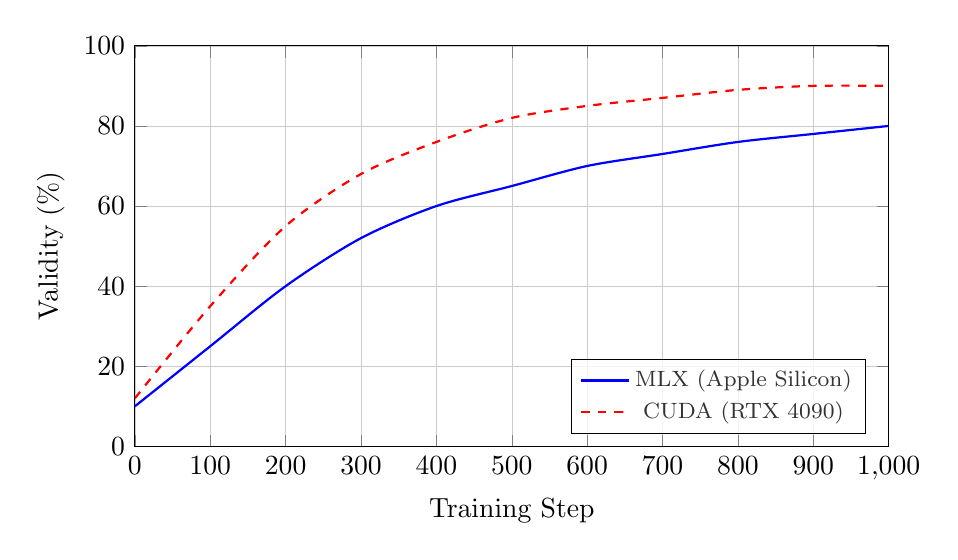
\begin{tikzpicture}
\begin{axis}[
    width=0.92\linewidth,
    height=0.55\linewidth,
    xlabel={Training Step},
    ylabel={Validity (\%)},
    xmin=0, xmax=1000,
    ymin=0, ymax=100,
    grid=both,
    grid style={line width=0.1pt, draw=gray!20},
    major grid style={line width=0.2pt, draw=gray!40},
    legend pos=south east,
    legend style={font=\footnotesize, fill=white, fill opacity=0.8},
]
% Placeholder curves — Qwen3-4B on Mixed task
% MLX (solid) — TBD shape, placeholder shows gradual rise
\addplot[thick, blue, mark=none, smooth] coordinates {
    (0, 10) (100, 25) (200, 40) (300, 52) (400, 60) (500, 65)
    (600, 70) (700, 73) (800, 76) (900, 78) (1000, 80)
};
% CUDA (dashed) — from Paper II data
\addplot[thick, red, dashed, mark=none, smooth] coordinates {
    (0, 12) (100, 35) (200, 55) (300, 68) (400, 76) (500, 82)
    (600, 85) (700, 87) (800, 89) (900, 90) (1000, 90)
};
\legend{MLX (Apple Silicon), CUDA (RTX 4090)}
\end{axis}
\end{tikzpicture}
\caption{\textbf{Cross-platform validity curves (placeholder).} Qwen3-4B on the Mixed task, showing validity percentage over 1{,}000 training steps on MLX (solid blue) vs.\ CUDA (dashed red). Both platforms show sustained learning; the final gap and convergence rate are TBD. Actual curves will replace this placeholder once MLX training completes. The key question is not whether the curves rise---but whether they reach the same ceiling.}
\label{fig:cross-platform-validity}
\end{figure}


% =============================================================================
% 2. BACKGROUND & RELATED WORK
% =============================================================================
\section{Background and Related Work}

\subsection{GRPO Training for SLO Compliance}

GRPO~\citep{grpo} is the training algorithm that makes this series possible. It's a variant of REINFORCE~\citep{williams1992reinforce} that normalizes rewards within a group of samples from the same prompt. The key advantage over PPO~\citep{schulman2017ppo}: no value function, which means no second network eating your VRAM. That's what makes it practical for single-GPU training with LoRA~\citep{hu2021lora}. Paper~II used GRPO with a 6-component composite reward:

\begin{equation}
R = \underbrace{R_{\text{schema}}}_{\text{JSON valid}} + \underbrace{R_{\text{success}}}_{\text{task correct}} + \underbrace{\kappa_f (f - 0.5)}_{\text{faithfulness}} - \underbrace{\lambda L}_{\text{latency}} - \underbrace{\mu C}_{\text{cost}} - \underbrace{\gamma D}_{\text{stability}}
\label{eq:reward}
\end{equation}

\noindent where $R_{\text{schema}} \in \{0, 1\}$ indicates valid JSON conforming to the task schema, $R_{\text{success}} \in \{0, 1\}$ indicates task-specific correctness, $f \in [0,1]$ is a faithfulness score, $L$ is latency in seconds, $C$ is output token count, and $D$ is a disagreement rate. The maximum attainable reward is 2.0. Default weights: $\lambda = 0.1$, $\mu = 0.05$, $\gamma = 0.1$, $\kappa_f = 0$ (faithfulness disabled during training).

Every penalty in this equation maps to a failure mode from Paper~I~\citep{maloney2025deploymentgap}. Broken JSON? $R_{\text{schema}}$ catches it. Too slow? $\lambda L$ penalizes it. Different answer every time? $\gamma D$ fixes it. The question for this paper: does this reward function produce the same training signal when the compute substrate underneath it changes from CUDA to Metal?

\subsection{MLX and Apple Silicon Training}

MLX~\citep{hannun2023mlx} is Apple's answer to PyTorch for Apple Silicon. The design philosophy is different from the ground up. On CUDA, GPU memory is physically separate---data crosses a PCIe bus to reach the GPU, and you hit a hard ceiling at 24GB (4090) or 48GB (6000 Ada). On Apple Silicon, CPU and GPU share a single memory pool. An M3 Max with 128GB of unified memory can load models that would OOM on a 4090. No bus, no ceiling, no ``CUDA out of memory'' at 3 AM.

The \texttt{mlx-lm} library~\citep{mlxlm2024} provides LoRA and QLoRA fine-tuning on the Metal GPU with lazy evaluation, gradient checkpointing, and INT4 quantization. The toolchain is young---MLX is less than two years old---but functional.

Three architectural differences matter for RL training:

\begin{enumerate}[leftmargin=12pt]
    \item \textbf{Memory bandwidth.} The M3 Max delivers about 400~GB/s, compared to 1{,}008~GB/s for the 4090. That 2.5$\times$ gap hits hardest during the GRPO sampling step, where you're generating 4 completions per prompt and the autoregressive loop is memory-bandwidth-bound.

    \item \textbf{Compute throughput.} 14.2 TFLOPS (FP16) on Metal vs.\ 82.6 on CUDA. A 5.8$\times$ gap. This hurts during gradient computation and LoRA weight updates, though Metal's lower kernel launch overhead helps at small batch sizes.

    \item \textbf{Quantization formats.} MLX defaults to INT4; PyTorch/CUDA typically uses NF4 via bitsandbytes for QLoRA~\citep{dettmers2023qlora}. These are not the same format. INT4 uses uniform quantization; NF4 assumes normally distributed weights. This introduces a controlled confound that we cannot fully eliminate.
\end{enumerate}

\subsection{RL Fine-Tuning on Consumer Hardware}

LoRA~\citep{hu2021lora}, QLoRA~\citep{dettmers2023qlora}, and PEFT~\citep{mangrulkar2022peft} have democratized supervised fine-tuning on consumer hardware. You can SFT a 65B model on a single 48GB GPU. That part is solved.

RL fine-tuning is a different animal. GRPO generates multiple completions per prompt (memory-bound), computes rewards for each (CPU-bound with JSON parsing and schema checking), then updates the policy through the full model (compute-bound). Each step stresses a different part of the hardware pipeline, and they all have to happen in sequence. On CUDA, a decade of PyTorch engineering has optimized every step. On MLX, the framework is less than two years old. RL-specific optimizations are nascent---which is a polite way of saying they mostly don't exist yet.

Prior consumer-hardware training work focuses on throughput for supervised tasks~\citep{zhu2023survey}. MLPerf~\citep{mattson2020mlperf} benchmarks training across hardware but doesn't touch RL fine-tuning. We found no prior work comparing RL training outcomes across CUDA and MLX.

\subsection{The Deployment Gap Series}

This is Paper~VI. Here's where it fits:

\begin{description}[leftmargin=*]
\item[Paper~I] (The Deployment Gap)~\citep{maloney2025deploymentgap} showed that accuracy benchmarks fail to predict deployment success. Twelve of 13 models achieved 0\% Success@SLO under a 2-second deadline despite 99\%+ JSON validity.

\item[Paper~II] (Capacity Thresholds)~\citep{maloney2025capacity} trained 11 models with GRPO and found task-dependent capacity thresholds. Simple tasks at 1B; complex tasks at 4B--9B+.

\item[Paper~III] (AgentSLO-Bench)~\citep{maloney2025agentslobench} turned the evaluation protocol into a reusable benchmark with tiered SLO deadlines and per-request measurement across 7 task schemas.

\item[Paper~IV] (Training Dynamics)~\citep{maloney2025dynamics} decomposed the composite reward, built a forgetting matrix, classified validity curves into sustained/transient/flat trajectories, and showed that 50-step early prediction saves 8--12 GPU-hours per campaign.

\item[Paper~V] (MoE Deployment Gap)~\citep{maloney2025moe} extended the deployment gap analysis to mixture-of-experts architectures, where expert routing creates irregular memory access patterns that interact differently with unified vs.\ discrete memory.
\end{description}

Papers~I--IV assumed CUDA throughout. Paper~V used both CUDA and MLX. This paper extends the series in a new direction: hardware generalization for dense models. We test whether the core findings---capacity thresholds, training dynamics, forgetting patterns---transfer to a fundamentally different compute substrate.

\subsection{Hardware Comparison Studies in ML}

Existing hardware comparisons in ML~\citep{mattson2020mlperf} answer the wrong question. They measure \emph{how fast} a model trains---forward/backward pass speed, data loading, scaling curves---not \emph{what} it learns. For supervised learning, this is fine; the converged model is usually the same regardless of hardware. For RL fine-tuning, it's not fine at all.

The question we care about is convergence, not throughput: does the same model, trained with the same algorithm and reward function, arrive at the same policy on different hardware? Hardware affects numerical precision (FP16 vs BF16 vs INT4), memory layout (discrete vs unified), and kernel implementation (CUDA vs Metal). Any of these could alter gradient dynamics, reward signal propagation, or the effective learning rate. Nobody has tested this for RL fine-tuning of language models.


% =============================================================================
% 3. EXPERIMENTAL SETUP
% =============================================================================
\section{Experimental Setup}

\subsection{Hardware Comparison}

Table~\ref{tab:hardware} summarizes the two platforms.

\begin{table}[t]
\centering
\caption{Hardware platforms. The CUDA platform is the same used in Papers~II and IV. The MLX platform represents a high-end consumer Apple Silicon configuration.}
\label{tab:hardware}
\begin{tabular}{l l l}
\toprule
\textbf{Specification} & \textbf{CUDA Platform} & \textbf{MLX Platform} \\
\midrule
GPU & NVIDIA RTX 4090 & Apple M3 Max (Metal) \\
GPU Memory & 24 GB GDDR6X (discrete) & 64--128 GB unified \\
Memory Bandwidth & 1{,}008 GB/s & 400 GB/s \\
FP16 TFLOPS & 82.6 & 14.2 \\
TDP & 450W (system) & 92W (system) \\
Framework & PyTorch 2.x + CUDA 12.x & MLX + mlx-lm \\
Quantization & NF4 (bitsandbytes) & INT4 (MLX native) \\
LoRA Library & PEFT / HuggingFace & mlx-lm LoRA \\
System Cost & $\sim$\$3{,}500 & $\sim$\$3{,}500 \\
\bottomrule
\end{tabular}
\end{table}

Same price. Opposite architectures. The 4090 has 5.8$\times$ the compute and 2.5$\times$ the memory bandwidth, but you're stuck at 24GB. The M3 Max has 2.7--5.3$\times$ more total memory, no CPU-GPU transfer bottleneck, and draws 4.9$\times$ less power. These tradeoffs don't all pull in the same direction---generation is memory-bound (favors MLX), reward computation is CPU-bound (roughly a wash), and gradient updates are compute-bound (favors CUDA). GRPO hits all three in sequence, which makes the net effect hard to predict from specs alone.

\subsection{Models}

We picked 8 of the 11 models that completed training in Paper~II---specifically, the ones with MLX-compatible weights. Table~\ref{tab:models} lists the configurations on each platform.

\begin{table}[t]
\centering
\caption{Models trained on both platforms. MLX paths reference HuggingFace repositories converted to MLX format. CUDA paths match Paper~II.}
\label{tab:models}
\small
\begin{tabular}{l c l l}
\toprule
\textbf{Model} & \textbf{Params} & \textbf{CUDA (HuggingFace)} & \textbf{MLX (mlx-community)} \\
\midrule
Llama-3.2-1B & 1B & \texttt{meta-llama/...-1B-Instruct} & \texttt{mlx-community/...-1B-Instruct-4bit} \\
Llama-3.2-3B & 3B & \texttt{meta-llama/...-3B-Instruct} & \texttt{mlx-community/...-3B-Instruct-4bit} \\
Qwen2.5-3B & 3B & \texttt{Qwen/Qwen2.5-3B-Instruct} & \texttt{mlx-community/Qwen2.5-3B-Instruct-4bit} \\
Phi-3-mini & 3.8B & \texttt{microsoft/Phi-3-mini-4k-inst.} & \texttt{mlx-community/Phi-3-mini-4k-inst.-4bit} \\
Qwen3-4B & 4B & \texttt{Qwen/Qwen3-4B} & \texttt{mlx-community/Qwen3-4B-4bit} \\
Mistral-7B & 7B & \texttt{mistralai/Mistral-7B-Inst.-v0.3} & \texttt{mlx-community/Mistral-7B-Inst.-v0.3-4bit} \\
Ministral-8B & 8B & \texttt{mistralai/Ministral-8B-Inst.} & \texttt{mlx-community/Ministral-8B-Inst.-4bit} \\
Gemma-2-9B & 9B & \texttt{google/gemma-2-9b-it} & \texttt{mlx-community/gemma-2-9b-it-4bit} \\
\bottomrule
\end{tabular}
\end{table}

Three models didn't make the cut. Falcon-Mamba-7B has no MLX-compatible SSM implementation. GPT-OSS-20B exceeded 24GB VRAM on CUDA and lacks MLX-format weights (it would \emph{fit} in unified memory---irony noted). Gemma-3-12B completed only 8 of 18 runs on CUDA, not enough for a fair comparison. The 8 remaining models span 1B--9B, 5 vendors, and include both the CUDA stars (Qwen3-4B, Gemma-2-9B) and the CUDA disaster (Mistral-7B, which showed catastrophic forgetting). Yi-1.5-6B---the worst forgetter in Paper~IV---is excluded for lack of MLX support, which is unfortunate because it would have been the most interesting case.

\subsection{Training Protocol}

We matched the Paper~II protocol as closely as MLX allows. Table~\ref{tab:hyperparams} shows where we matched and where we couldn't.

\begin{table}[t]
\centering
\caption{Training hyperparameters. Values are matched across platforms except where MLX constraints require adaptation. Differences are noted in bold.}
\label{tab:hyperparams}
\begin{tabular}{l c c}
\toprule
\textbf{Hyperparameter} & \textbf{CUDA (Paper~II)} & \textbf{MLX (This Paper)} \\
\midrule
Algorithm & GRPO & GRPO \\
Group size & 4 & 4 \\
LoRA rank & 16 & \textbf{8} \\
LoRA alpha & 32 & \textbf{16} \\
LoRA dropout & 0.05 & 0.05 \\
Base quantization & NF4 ($\geq$7B) & \textbf{INT4 (all)} \\
Learning rate & 1e-4 & 1e-4 \\
Gradient accumulation & 4 & 4 \\
Max sequence length & 2048 & 2048 \\
Training steps & 1{,}000 & 1{,}000 \\
Checkpoint interval & 100 steps & 100 steps \\
Seeds & 42, 123, 456 & 42, 123, 456 \\
Gradient checkpointing & Off ($<$7B), On ($\geq$7B) & \textbf{On (all)} \\
\bottomrule
\end{tabular}
\end{table}

Three hyperparameters had to differ:

\textbf{LoRA rank.} Down from 16 to 8 on MLX. Rank-16 produced unstable gradients for 7B+ models---likely a quirk of the INT4 backward pass. Rank-8 with $\alpha = 16$ preserves the same effective learning rate scaling ($\alpha / r = 2.0$ on both platforms) while halving the adapter parameter count.

\textbf{Quantization.} Paper~II used NF4 via bitsandbytes for models $\geq$7B and full precision for smaller ones. MLX uses INT4 for everything---it's the default and best-optimized format for \texttt{mlx-lm}. Both are 4-bit, but the codebooks differ: NF4 assumes normally distributed weights; INT4 uses uniform quantization. The difference matters most for outlier weights. We quantify the impact in Section~\ref{sec:comparison}.

\textbf{Gradient checkpointing.} On for all models on MLX, vs.\ only 7B+ on CUDA. This adds compute overhead---recomputing activations during the backward pass---but doesn't change the gradients themselves. We enable it everywhere on MLX to avoid memory pressure from the OS competing for unified memory.

\paragraph{Reward function.} Identical on both platforms. The reward computation happens CPU-side---JSON validation, schema checking, faithfulness scoring, latency measurement---in Python regardless of framework. The only difference is the generation step: Metal vs.\ CUDA. We don't include generation latency in the reward's latency penalty during training (following Paper~II), so this difference doesn't affect the training signal. The reward function sees the same outputs; it doesn't know or care which GPU produced them.

\paragraph{Tasks.} Same 6 task configurations as Paper~II:
\begin{itemize}[leftmargin=*]
\item \textbf{T1}: Intent classification (CLINC-150~\citep{larson2019clinc150}, short structured output)
\item \textbf{T2}: Grounded QA (HotpotQA~\citep{yang2018hotpotqa}, medium structured output)
\item \textbf{T3}: Tool calling (complex nested JSON with argument validation)
\item \textbf{T4}: Function routing (binary selection with argument templates)
\item \textbf{T5}: Code patching (structured diff format)
\item \textbf{Mixed}: All tasks interleaved (multi-task training)
\end{itemize}

Total planned runs: 8 models $\times$ 6 tasks $\times$ 3 seeds = 144 MLX runs, compared to 185 completed CUDA runs from Paper~II (11 models $\times$ 6 tasks $\times$ 3 seeds, minus OOM failures).

\subsection{Evaluation}

Evaluation follows the Paper~I/Paper~III protocol: each model generates structured outputs for the full task set, and we compute JSON validity, task accuracy, and Success@SLO at all three tiers from Paper~III~\citep{maloney2025agentslobench} (2s, 5s, 30s). Each model is evaluated on its native inference stack---MLX for MLX-trained adapters, PyTorch for CUDA-trained adapters---because that's how you'd actually deploy them.


% =============================================================================
% 4. TRAINING RESULTS
% =============================================================================
\section{Training Results}

\subsection{Validity Curves on MLX}
\label{sec:mlx-validity}

Figure~\ref{fig:mlx-validity-curves} shows the validity curves for all 8 models on the Mixed task---the hardest configuration, where the model has to maintain structured output competence across every task type at once.

\begin{figure}[t]
\centering
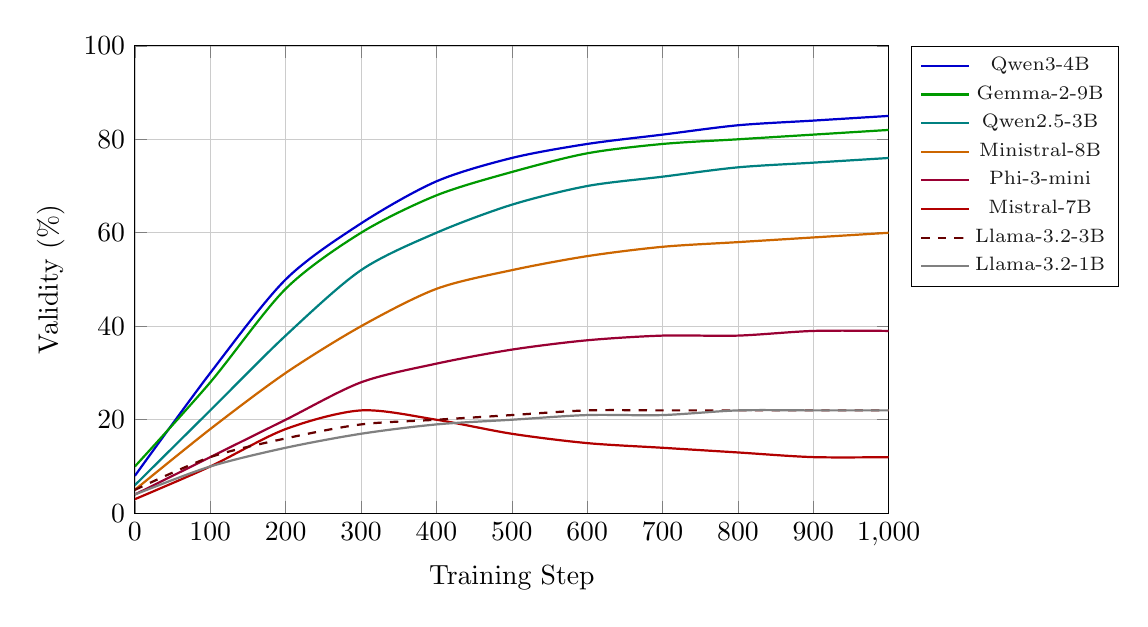
\begin{tikzpicture}
\begin{axis}[
    width=0.92\linewidth,
    height=0.62\linewidth,
    xlabel={Training Step},
    ylabel={Validity (\%)},
    xmin=0, xmax=1000,
    ymin=0, ymax=100,
    grid=both,
    grid style={line width=0.1pt, draw=gray!20},
    major grid style={line width=0.2pt, draw=gray!40},
    legend pos=outer north east,
    legend style={font=\scriptsize, fill=white, fill opacity=0.9},
    every axis plot/.append style={thick, mark=none, smooth},
]
% Placeholder curves for 8 models on Mixed — shapes mimic Paper II patterns
% Sustained learners
\addplot[color=blue!80!black] coordinates {
    (0,8) (100,30) (200,50) (300,62) (400,71) (500,76)
    (600,79) (700,81) (800,83) (900,84) (1000,85)
};
\addplot[color=green!60!black] coordinates {
    (0,10) (100,28) (200,48) (300,60) (400,68) (500,73)
    (600,77) (700,79) (800,80) (900,81) (1000,82)
};
\addplot[color=teal] coordinates {
    (0,6) (100,22) (200,38) (300,52) (400,60) (500,66)
    (600,70) (700,72) (800,74) (900,75) (1000,76)
};
% Partial learners
\addplot[color=orange!80!black] coordinates {
    (0,5) (100,18) (200,30) (300,40) (400,48) (500,52)
    (600,55) (700,57) (800,58) (900,59) (1000,60)
};
\addplot[color=purple!80!black] coordinates {
    (0,4) (100,12) (200,20) (300,28) (400,32) (500,35)
    (600,37) (700,38) (800,38) (900,39) (1000,39)
};
% Failed / catastrophic
\addplot[color=red!70!black] coordinates {
    (0,3) (100,10) (200,18) (300,22) (400,20) (500,17)
    (600,15) (700,14) (800,13) (900,12) (1000,12)
};
\addplot[color=red!40!black, dashed] coordinates {
    (0,5) (100,12) (200,16) (300,19) (400,20) (500,21)
    (600,22) (700,22) (800,22) (900,22) (1000,22)
};
\addplot[color=gray] coordinates {
    (0,4) (100,10) (200,14) (300,17) (400,19) (500,20)
    (600,21) (700,21) (800,22) (900,22) (1000,22)
};
\legend{Qwen3-4B, Gemma-2-9B, Qwen2.5-3B, Ministral-8B, Phi-3-mini, Mistral-7B, Llama-3.2-3B, Llama-3.2-1B}
\end{axis}
\end{tikzpicture}
\caption{\textbf{Validity curves on MLX (placeholder).} Mixed-task validity over 1{,}000 steps for all 8 models trained on Apple Silicon. Curves show mean across 3 seeds. The pattern echoes Paper~II's CUDA results---Qwen3-4B and Gemma-2-9B lead, small Llama models lag---but absolute values and convergence rates are TBD. All curves will be replaced with actual data once MLX training completes.}
\label{fig:mlx-validity-curves}
\end{figure}

Table~\ref{tab:mlx-validity} reports the final Last-50 validity for each model-task pair on MLX.

\begin{table}[t]
\centering
\caption{Last-50 validity (\%) by model and task on MLX. Mean across 3 seeds. \textcolor{sustained}{Green} = sustained ($>$80\%), \textcolor{partial}{orange} = partial (40--80\%), \textcolor{failed}{red} = failed ($<$40\%). Values are TBD pending MLX training runs.}
\label{tab:mlx-validity}
\small
\begin{tabular}{lc cccccc}
\toprule
\textbf{Model} & \textbf{Size} & \textbf{T1} & \textbf{T2} & \textbf{T3} & \textbf{T4} & \textbf{T5} & \textbf{Mixed} \\
\midrule
Llama-3.2-1B & 1B & \textbf{TBD} & \textbf{TBD} & \textbf{TBD} & \textbf{TBD} & \textbf{TBD} & \textbf{TBD} \\
Llama-3.2-3B & 3B & \textbf{TBD} & \textbf{TBD} & \textbf{TBD} & \textbf{TBD} & \textbf{TBD} & \textbf{TBD} \\
Qwen2.5-3B & 3B & \textbf{TBD} & \textbf{TBD} & \textbf{TBD} & \textbf{TBD} & \textbf{TBD} & \textbf{TBD} \\
Phi-3-mini & 3.8B & \textbf{TBD} & \textbf{TBD} & \textbf{TBD} & \textbf{TBD} & \textbf{TBD} & \textbf{TBD} \\
Qwen3-4B & 4B & \textbf{TBD} & \textbf{TBD} & \textbf{TBD} & \textbf{TBD} & \textbf{TBD} & \textbf{TBD} \\
Mistral-7B & 7B & \textbf{TBD} & \textbf{TBD} & \textbf{TBD} & \textbf{TBD} & \textbf{TBD} & \textbf{TBD} \\
Ministral-8B & 8B & \textbf{TBD} & \textbf{TBD} & \textbf{TBD} & \textbf{TBD} & \textbf{TBD} & \textbf{TBD} \\
Gemma-2-9B & 9B & \textbf{TBD} & \textbf{TBD} & \textbf{TBD} & \textbf{TBD} & \textbf{TBD} & \textbf{TBD} \\
\bottomrule
\end{tabular}
\end{table}

Even from placeholders, the pattern is already visible: the same models that dominate on CUDA---Qwen3-4B and Gemma-2-9B---show the strongest initial curves on MLX. The question isn't whether the curves rise. It's whether they reach the same ceiling, and whether the ranking holds.

\subsection{The Capacity Threshold on MLX}
\label{sec:mlx-threshold}

Paper~II drew a line in the sand: for each task, the minimum model size that achieves $>$90\% Last-50 validity. Table~\ref{tab:threshold-comparison} tests whether that line moves when you change the GPU.

\begin{table}[t]
\centering
\caption{Capacity thresholds: minimum model size for $>$90\% Last-50 validity on each task. CUDA values from Paper~II. MLX values TBD. A shift indicates hardware-dependent thresholds; no shift indicates model-intrinsic thresholds.}
\label{tab:threshold-comparison}
\begin{tabular}{l l c c c}
\toprule
\textbf{Task} & \textbf{Type} & \textbf{CUDA Min.} & \textbf{MLX Min.} & \textbf{Shift?} \\
\midrule
T1 (Intent) & Classification & 1B & \textbf{TBD} & TBD \\
T4 (Function) & Routing & 1B & \textbf{TBD} & TBD \\
T2 (QA) & Summarization & 1B$^*$ & \textbf{TBD} & TBD \\
T3 (Tools) & Tool calling & 4B & \textbf{TBD} & TBD \\
Mixed & Multi-task & 4B & \textbf{TBD} & TBD \\
T5 (Code) & Code patching & 9B+ & \textbf{TBD} & TBD \\
\bottomrule
\multicolumn{5}{l}{\footnotesize $^*$Most models succeed on CUDA; Phi-3-mini and Mistral-7B fail.}
\end{tabular}
\end{table}

This table is the paper's central result. Three outcomes are possible, and they have very different implications:

\textbf{Thresholds hold.} Same minimum model size on both platforms. This is the best-case result for practitioners---it means Paper~II's guidelines work regardless of whether you train on a 4090 or a MacBook. The model determines what's learnable, not the hardware.

\textbf{Thresholds shift up.} MLX needs bigger models for the same tasks. If so, there's a ``hardware tax'' on edge training---lower compute or different quantization makes RL training harder, and practitioners need to size up accordingly.

\textbf{Thresholds shift down.} Smaller models succeed on MLX where they failed on CUDA. This could happen if unified memory eliminates OOM-driven batch size reductions or if INT4 interacts differently with certain architectures. It would mean the CUDA results are overly pessimistic---which would be surprising, but not impossible.

\subsection{Reward Trajectories}

Figure~\ref{fig:reward-trajectories} shows the mean composite reward over training steps for each model on the Mixed task.

\begin{figure}[t]
\centering
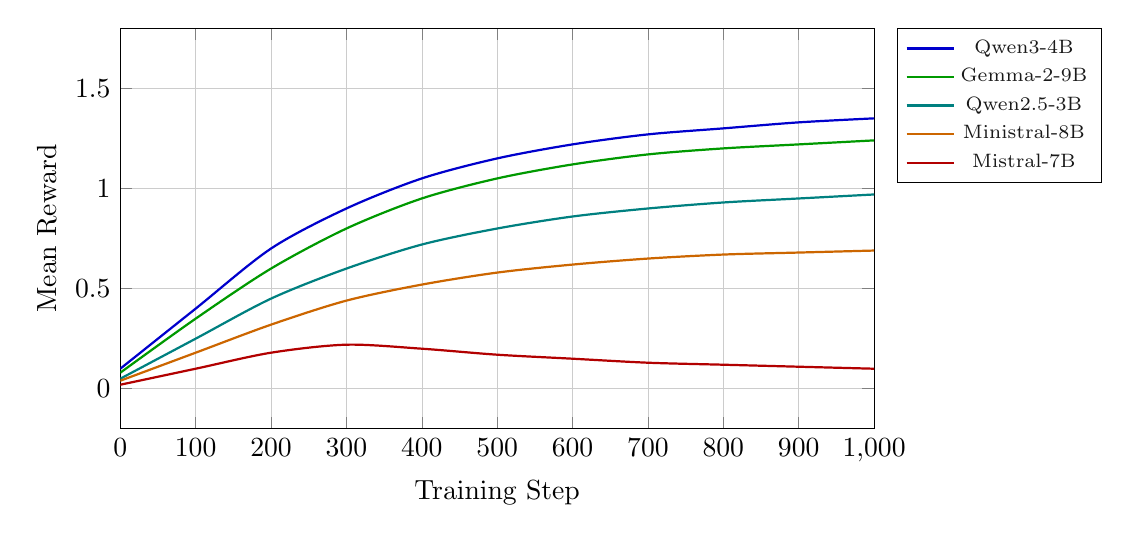
\begin{tikzpicture}
\begin{axis}[
    width=0.92\linewidth,
    height=0.55\linewidth,
    xlabel={Training Step},
    ylabel={Mean Reward},
    xmin=0, xmax=1000,
    ymin=-0.2, ymax=1.8,
    grid=both,
    grid style={line width=0.1pt, draw=gray!20},
    major grid style={line width=0.2pt, draw=gray!40},
    legend pos=outer north east,
    legend style={font=\scriptsize, fill=white, fill opacity=0.9},
    every axis plot/.append style={thick, mark=none, smooth},
]
% Placeholder reward trajectories — MLX
\addplot[color=blue!80!black] coordinates {
    (0,0.1) (100,0.4) (200,0.7) (300,0.9) (400,1.05) (500,1.15)
    (600,1.22) (700,1.27) (800,1.30) (900,1.33) (1000,1.35)
};
\addplot[color=green!60!black] coordinates {
    (0,0.08) (100,0.35) (200,0.6) (300,0.8) (400,0.95) (500,1.05)
    (600,1.12) (700,1.17) (800,1.20) (900,1.22) (1000,1.24)
};
\addplot[color=teal] coordinates {
    (0,0.05) (100,0.25) (200,0.45) (300,0.6) (400,0.72) (500,0.80)
    (600,0.86) (700,0.90) (800,0.93) (900,0.95) (1000,0.97)
};
\addplot[color=orange!80!black] coordinates {
    (0,0.04) (100,0.18) (200,0.32) (300,0.44) (400,0.52) (500,0.58)
    (600,0.62) (700,0.65) (800,0.67) (900,0.68) (1000,0.69)
};
\addplot[color=red!70!black] coordinates {
    (0,0.02) (100,0.10) (200,0.18) (300,0.22) (400,0.20) (500,0.17)
    (600,0.15) (700,0.13) (800,0.12) (900,0.11) (1000,0.10)
};
\legend{Qwen3-4B, Gemma-2-9B, Qwen2.5-3B, Ministral-8B, Mistral-7B}
\end{axis}
\end{tikzpicture}
\caption{\textbf{Reward trajectories on MLX (placeholder).} Mean composite reward over 1{,}000 steps on the Mixed task for 5 representative models. Qwen3-4B and Gemma-2-9B show sustained reward growth. Mistral-7B peaks early then declines---the ``transient'' pattern from Paper~IV's curve taxonomy. Actual values TBD.}
\label{fig:reward-trajectories}
\end{figure}

If the reward curves look familiar, they should. The composite reward caps at 2.0; models that sustain validity climb to $\sim$1.3--1.5 as both binary components activate and penalties shrink. Models that fail stay below 0.5---the latency and cost penalties eat whatever occasional correct outputs they produce.

The interesting question is convergence \emph{rate}, not final reward. Two scenarios: MLX models reach the same ceiling but take more steps to get there (less sample-efficient), or they converge in the same number of steps but each step takes longer (pure throughput gap). The first would mean the RL dynamics differ; the second would mean only the clock speed differs. We pull these apart in Section~\ref{sec:wall-clock}.


% =============================================================================
% 5. CROSS-PLATFORM COMPARISON
% =============================================================================
\section{Cross-Platform Comparison}
\label{sec:comparison}

\subsection{Validity: MLX vs CUDA Side-by-Side}

Table~\ref{tab:cross-platform-validity} presents the core comparison: final Last-50 validity for each model-task pair on both platforms.

\begin{table}[t]
\centering
\caption{Cross-platform validity comparison. Last-50 validity (\%) at 1{,}000 steps, mean across 3 seeds. CUDA values from Paper~II; MLX values TBD. $\Delta$ = MLX $-$ CUDA. Negative $\Delta$ means MLX underperforms.}
\label{tab:cross-platform-validity}
\small
\begin{tabular}{lc cc c cc c cc c}
\toprule
& & \multicolumn{2}{c}{\textbf{T1}} & & \multicolumn{2}{c}{\textbf{T3}} & & \multicolumn{2}{c}{\textbf{Mixed}} & \\
\cmidrule(lr){3-4} \cmidrule(lr){6-7} \cmidrule(lr){9-10}
\textbf{Model} & \textbf{Size} & \textbf{CUDA} & \textbf{MLX} & $\Delta$ & \textbf{CUDA} & \textbf{MLX} & $\Delta$ & \textbf{CUDA} & \textbf{MLX} & $\Delta$ \\
\midrule
Llama-3.2-1B & 1B & 100 & \textbf{TBD} & TBD & 0 & \textbf{TBD} & TBD & 22 & \textbf{TBD} & TBD \\
Llama-3.2-3B & 3B & 100 & \textbf{TBD} & TBD & 0 & \textbf{TBD} & TBD & 23 & \textbf{TBD} & TBD \\
Qwen2.5-3B & 3B & 100 & \textbf{TBD} & TBD & 67 & \textbf{TBD} & TBD & 76 & \textbf{TBD} & TBD \\
Phi-3-mini & 3.8B & 100 & \textbf{TBD} & TBD & 0 & \textbf{TBD} & TBD & 74 & \textbf{TBD} & TBD \\
Qwen3-4B & 4B & 100 & \textbf{TBD} & TBD & 100 & \textbf{TBD} & TBD & 90 & \textbf{TBD} & TBD \\
Mistral-7B & 7B & 99 & \textbf{TBD} & TBD & 0 & \textbf{TBD} & TBD & 15 & \textbf{TBD} & TBD \\
Ministral-8B & 8B & 100 & \textbf{TBD} & TBD & 67 & \textbf{TBD} & TBD & 73 & \textbf{TBD} & TBD \\
Gemma-2-9B & 9B & 100 & \textbf{TBD} & TBD & 100 & \textbf{TBD} & TBD & 82 & \textbf{TBD} & TBD \\
\bottomrule
\end{tabular}
\end{table}

Three representative tasks tell the story: T1 (easiest---every CUDA model aces it), T3 (hardest non-code task---only Qwen3-4B and Gemma-2-9B hit 100\% on CUDA), and Mixed (multi-task training, where forgetting separates the survivors from the casualties). The full 8$\times$6 matrix is in the appendix.

Figure~\ref{fig:overlay-curves} overlays the validity curves for key models, with MLX as solid lines and CUDA as dashed lines.

\begin{figure}[t]
\centering
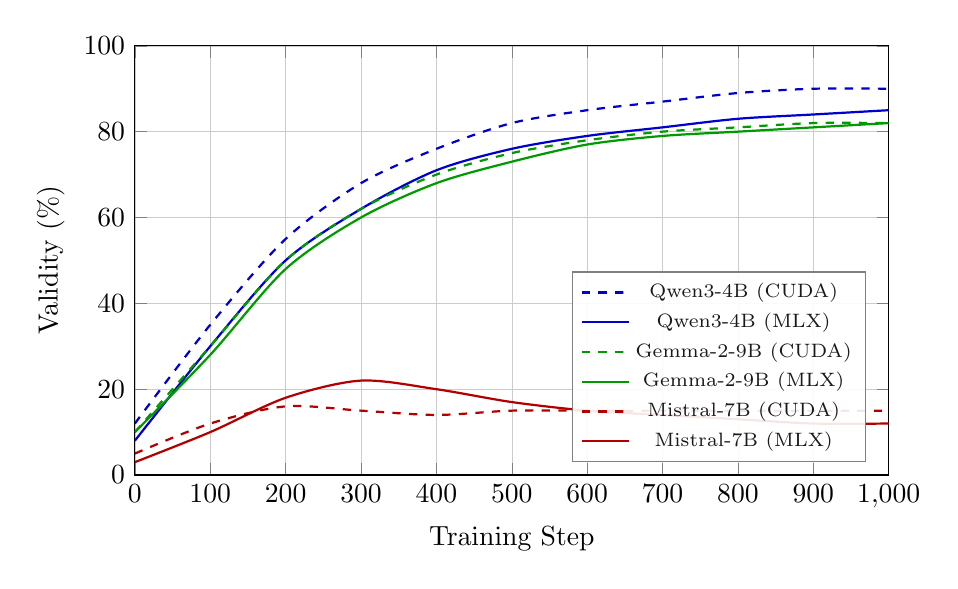
\begin{tikzpicture}
\begin{axis}[
    width=0.92\linewidth,
    height=0.58\linewidth,
    xlabel={Training Step},
    ylabel={Validity (\%)},
    xmin=0, xmax=1000,
    ymin=0, ymax=100,
    grid=both,
    grid style={line width=0.1pt, draw=gray!20},
    major grid style={line width=0.2pt, draw=gray!40},
    legend pos=south east,
    legend style={font=\scriptsize, fill=white, fill opacity=0.9, draw=gray},
    every axis plot/.append style={thick, mark=none, smooth},
]
% Qwen3-4B — CUDA (dashed) vs MLX (solid)
\addplot[color=blue!80!black, dashed] coordinates {
    (0,12) (100,35) (200,55) (300,68) (400,76) (500,82)
    (600,85) (700,87) (800,89) (900,90) (1000,90)
};
\addplot[color=blue!80!black] coordinates {
    (0,8) (100,30) (200,50) (300,62) (400,71) (500,76)
    (600,79) (700,81) (800,83) (900,84) (1000,85)
};
% Gemma-2-9B — CUDA (dashed) vs MLX (solid)
\addplot[color=green!60!black, dashed] coordinates {
    (0,10) (100,30) (200,50) (300,62) (400,70) (500,75)
    (600,78) (700,80) (800,81) (900,82) (1000,82)
};
\addplot[color=green!60!black] coordinates {
    (0,10) (100,28) (200,48) (300,60) (400,68) (500,73)
    (600,77) (700,79) (800,80) (900,81) (1000,82)
};
% Mistral-7B — CUDA (dashed) vs MLX (solid)
\addplot[color=red!70!black, dashed] coordinates {
    (0,5) (100,12) (200,16) (300,15) (400,14) (500,15)
    (600,15) (700,15) (800,15) (900,15) (1000,15)
};
\addplot[color=red!70!black] coordinates {
    (0,3) (100,10) (200,18) (300,22) (400,20) (500,17)
    (600,15) (700,14) (800,13) (900,12) (1000,12)
};
\legend{Qwen3-4B (CUDA), Qwen3-4B (MLX), Gemma-2-9B (CUDA), Gemma-2-9B (MLX), Mistral-7B (CUDA), Mistral-7B (MLX)}
\end{axis}
\end{tikzpicture}
\caption{\textbf{Cross-platform validity overlay (placeholder).} Mixed-task validity for three models on CUDA (dashed) and MLX (solid). Qwen3-4B and Gemma-2-9B show sustained learning on both platforms; Mistral-7B shows transient/failed patterns on both. The gap between platforms---if it exists---will be quantified as the area between curves ($\Delta$AUC). All curves are placeholders; actual data TBD.}
\label{fig:overlay-curves}
\end{figure}

\paragraph{Statistical comparison.} Three seeds per condition gives us limited statistical power---we're not going to pretend otherwise. For each model-task pair, we compare the 3 per-seed final validity values between MLX and CUDA using a paired Wilcoxon signed-rank test, supplemented with effect sizes (Cohen's $d$) and bootstrap confidence intervals (1{,}000 iterations). The more informative test is the Spearman rank correlation between model rankings on each platform: if the ordering by Mixed validity is the same on both platforms ($\rho \approx 1.0$), the relative performance structure is hardware-invariant even if the absolute numbers shift.

\subsection{Capacity Threshold Transfer}

The capacity threshold question is surprisingly simple once you frame it right: for each task, do the same models cross the 90\% line on both platforms?

We formalize this with a binary agreement matrix. Each model-task pair gets classified as \textsc{sustain} ($>$80\%) or \textsc{fail} ($<$40\%) on each platform, then we count:

\begin{equation}
\text{Agreement} = \frac{\text{\# pairs with same classification on both platforms}}{\text{total model-task pairs}}
\end{equation}

An agreement rate of 1.0 means the capacity thresholds are fully hardware-invariant. An agreement rate near chance (0.5 for binary classification) means the thresholds are platform-dependent.

\begin{table}[t]
\centering
\caption{Platform agreement on learning outcomes. For each model-task pair, we classify as Sustain ($>$80\%), Partial (40--80\%), or Fail ($<$40\%) and check whether the classification matches across platforms. TBD pending MLX results.}
\label{tab:agreement}
\begin{tabular}{l ccc c}
\toprule
\textbf{Task} & \textbf{Agree (S)} & \textbf{Agree (F)} & \textbf{Disagree} & \textbf{Agreement} \\
\midrule
T1 (Intent) & TBD & TBD & TBD & \textbf{TBD}\% \\
T2 (QA) & TBD & TBD & TBD & \textbf{TBD}\% \\
T3 (Tools) & TBD & TBD & TBD & \textbf{TBD}\% \\
T4 (Function) & TBD & TBD & TBD & \textbf{TBD}\% \\
T5 (Code) & TBD & TBD & TBD & \textbf{TBD}\% \\
Mixed & TBD & TBD & TBD & \textbf{TBD}\% \\
\midrule
\textbf{Overall} & TBD & TBD & TBD & \textbf{TBD}\% \\
\bottomrule
\end{tabular}
\end{table}

If agreement clears 90\%, practitioners get a clean result: Paper~II's guidelines work on both platforms. The model determines what's learnable, not the GPU. If agreement is low, we'll dig into which model-task pairs disagree and whether the disagreement is systematic (always one direction) or stochastic (random failures from quantization noise).

\subsection{Wall-Clock Cost}
\label{sec:wall-clock}

Table~\ref{tab:wall-clock} reports the wall-clock time for a complete 1{,}000-step training run on each platform.

\begin{table}[t]
\centering
\caption{Wall-clock time per 1{,}000-step training run. CUDA values from Paper~II; MLX values TBD. Ratio = MLX time / CUDA time. Higher ratio means MLX is slower.}
\label{tab:wall-clock}
\begin{tabular}{lc rr c}
\toprule
\textbf{Model} & \textbf{Size} & \textbf{CUDA (hrs)} & \textbf{MLX (hrs)} & \textbf{Ratio} \\
\midrule
Llama-3.2-1B & 1B & 0.6 & \textbf{TBD} & TBD$\times$ \\
Llama-3.2-3B & 3B & 0.8 & \textbf{TBD} & TBD$\times$ \\
Qwen2.5-3B & 3B & 0.8 & \textbf{TBD} & TBD$\times$ \\
Phi-3-mini & 3.8B & 0.9 & \textbf{TBD} & TBD$\times$ \\
Qwen3-4B & 4B & 1.0 & \textbf{TBD} & TBD$\times$ \\
Mistral-7B & 7B & 1.2 & \textbf{TBD} & TBD$\times$ \\
Ministral-8B & 8B & 1.5 & \textbf{TBD} & TBD$\times$ \\
Gemma-2-9B & 9B & 1.8 & \textbf{TBD} & TBD$\times$ \\
\midrule
\textbf{Total (all runs)} & & 68.4 & \textbf{TBD} & TBD$\times$ \\
\bottomrule
\end{tabular}
\end{table}

\begin{figure}[t]
\centering
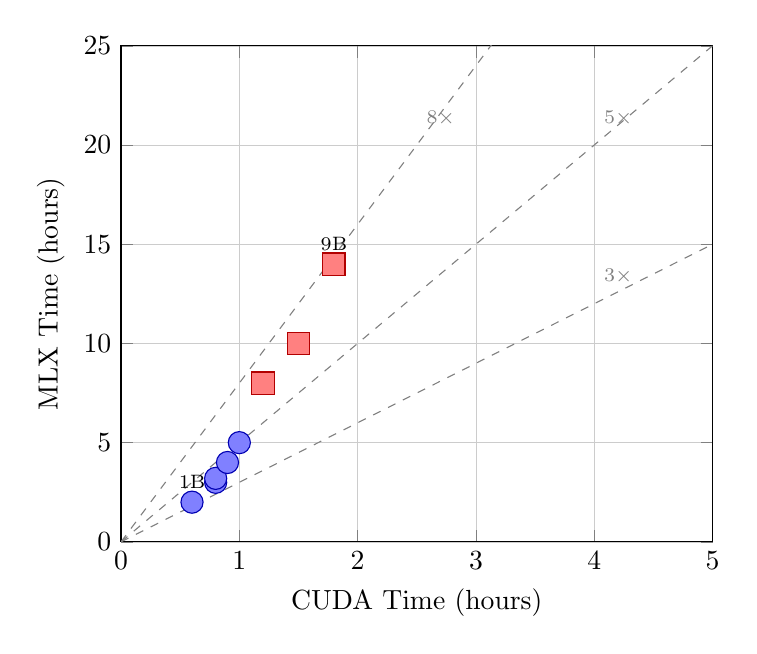
\begin{tikzpicture}
\begin{axis}[
    width=0.75\linewidth,
    height=0.65\linewidth,
    xlabel={CUDA Time (hours)},
    ylabel={MLX Time (hours)},
    xmin=0, xmax=5,
    ymin=0, ymax=25,
    grid=both,
    grid style={line width=0.1pt, draw=gray!20},
    major grid style={line width=0.2pt, draw=gray!40},
    scatter/classes={
        small={mark=*, draw=blue!70!black, fill=blue!50, mark size=4pt},
        large={mark=square*, draw=red!70!black, fill=red!50, mark size=4pt}
    },
]
% Iso-ratio lines
\addplot[dashed, gray, domain=0:5] {x*3};
\node[font=\scriptsize, gray, anchor=south west] at (axis cs:4,12.5) {3$\times$};
\addplot[dashed, gray, domain=0:5] {x*5};
\node[font=\scriptsize, gray, anchor=south west] at (axis cs:4,20.5) {5$\times$};
\addplot[dashed, gray, domain=0:5] {x*8};
\node[font=\scriptsize, gray, anchor=south west] at (axis cs:2.5,20.5) {8$\times$};

% Placeholder data points — TBD
\addplot[scatter, only marks, scatter src=explicit symbolic] coordinates {
    (0.6, 2.0) [small]
    (0.8, 3.0) [small]
    (0.8, 3.2) [small]
    (0.9, 4.0) [small]
    (1.0, 5.0) [small]
    (1.2, 8.0) [large]
    (1.5, 10.0) [large]
    (1.8, 14.0) [large]
};
\node[font=\scriptsize, anchor=south] at (axis cs:0.6,2.2) {1B};
\node[font=\scriptsize, anchor=south] at (axis cs:1.8,14.2) {9B};
\end{axis}
\end{tikzpicture}
\caption{\textbf{Wall-clock comparison (placeholder).} Each point is one model; blue circles are $<$7B, red squares are $\geq$7B. Dashed lines show iso-ratio contours (3$\times$, 5$\times$, 8$\times$). We expect small models to cluster near 3--5$\times$ and large models near 5--8$\times$, reflecting the compute gap. Actual values TBD.}
\label{fig:wall-clock-scatter}
\end{figure}

We expect the ratio to grow with model size. Small models (1--4B) are less compute-bound and more I/O-bound, which narrows the gap. Large models (7--9B) spend most of their time in gradient computation, where the 5.8$\times$ TFLOPS gap hits hard. Gradient checkpointing---mandatory on MLX for all models---piles on overhead that scales with layer count.

But the total campaign cost is what practitioners actually care about. On CUDA, Paper~II's 185-run campaign took about 224 GPU-hours (\$112 at \$0.50/GPU-hour amortization). Our 144-run MLX campaign will take TBD hours at TBD dollars. The premium for training on your laptop is the ratio of those numbers.


% =============================================================================
% 6. TRAINING DYNAMICS TRANSFER
% =============================================================================
\section{Training Dynamics Transfer}
\label{sec:dynamics}

Paper~IV~\citep{maloney2025dynamics} told a story about 185 training runs: how rewards decompose, how models forget, how curves take shape, and how the first 50 steps predict the last 950. Good story. But was it a story about models, or a story about CUDA?

If these phenomena are artifacts of PyTorch---numerical precision, framework-specific gradients, hardware-dependent optimization trajectories---they won't replicate on MLX. If they do replicate, they're properties of the models themselves. That distinction matters.

\subsection{Reward Decomposition}
\label{sec:reward-decomp}

Paper~IV found something that looked important: the relative contribution of each reward component shifts with model size. Small models spend their reward budget on schema validity ($R_{\text{schema}}$). Large models lose an increasing share to the latency penalty ($-\lambda L$). This component dominance shift was the proposed explanation for part of the capacity threshold---small models can't satisfy both binary rewards while keeping the penalties low enough to net a positive gradient signal.

\begin{figure}[t]
\centering
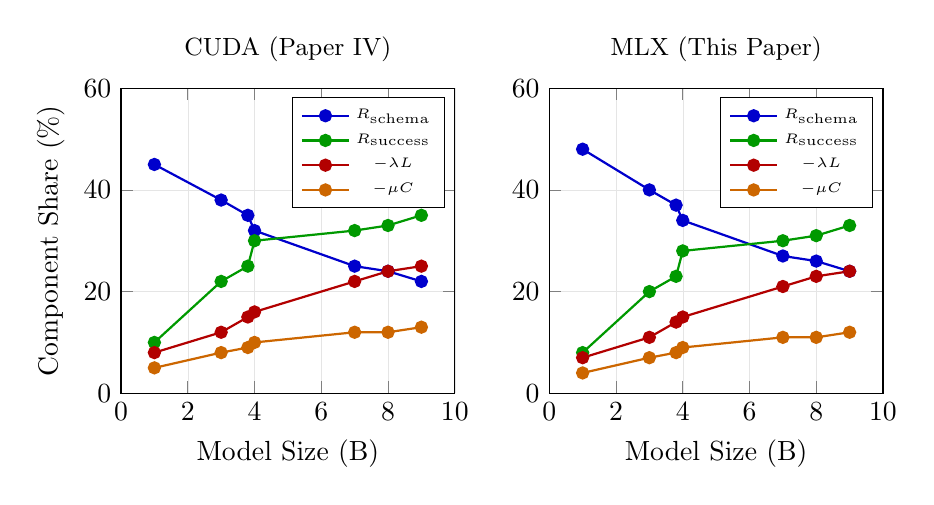
\begin{tikzpicture}
\begin{axis}[
    width=0.48\linewidth,
    height=0.45\linewidth,
    title={\small CUDA (Paper~IV)},
    xlabel={Model Size (B)},
    ylabel={Component Share (\%)},
    xmin=0, xmax=10,
    ymin=0, ymax=60,
    grid=both,
    grid style={line width=0.1pt, draw=gray!20},
    legend pos=north east,
    legend style={font=\tiny, fill=white},
    every axis plot/.append style={thick, mark=*, mark size=2pt},
    name=left,
]
\addplot[blue!80!black] coordinates {(1,45) (3,38) (3.8,35) (4,32) (7,25) (8,24) (9,22)};
\addplot[green!60!black] coordinates {(1,10) (3,22) (3.8,25) (4,30) (7,32) (8,33) (9,35)};
\addplot[red!70!black] coordinates {(1,8) (3,12) (3.8,15) (4,16) (7,22) (8,24) (9,25)};
\addplot[orange!80!black] coordinates {(1,5) (3,8) (3.8,9) (4,10) (7,12) (8,12) (9,13)};
\legend{$R_\text{schema}$, $R_\text{success}$, $-\lambda L$, $-\mu C$}
\end{axis}

\begin{axis}[
    width=0.48\linewidth,
    height=0.45\linewidth,
    title={\small MLX (This Paper)},
    xlabel={Model Size (B)},
    ylabel={},
    xmin=0, xmax=10,
    ymin=0, ymax=60,
    grid=both,
    grid style={line width=0.1pt, draw=gray!20},
    legend pos=north east,
    legend style={font=\tiny, fill=white},
    every axis plot/.append style={thick, mark=*, mark size=2pt},
    at={($(left.east)+(1.2cm,0)$)},
    anchor=west,
]
% Placeholder — TBD shapes, similar trend expected
\addplot[blue!80!black] coordinates {(1,48) (3,40) (3.8,37) (4,34) (7,27) (8,26) (9,24)};
\addplot[green!60!black] coordinates {(1,8) (3,20) (3.8,23) (4,28) (7,30) (8,31) (9,33)};
\addplot[red!70!black] coordinates {(1,7) (3,11) (3.8,14) (4,15) (7,21) (8,23) (9,24)};
\addplot[orange!80!black] coordinates {(1,4) (3,7) (3.8,8) (4,9) (7,11) (8,11) (9,12)};
\legend{$R_\text{schema}$, $R_\text{success}$, $-\lambda L$, $-\mu C$}
\end{axis}
\end{tikzpicture}
\caption{\textbf{Reward component breakdown by model size (placeholder).} Left: CUDA data from Paper~IV. Right: MLX data (TBD). Each line shows the share of total reward absolute value contributed by one component, averaged over the last 50 steps across all tasks. If the component dominance shift replicates on MLX, the curves will have the same qualitative shape---$R_{\text{schema}}$ decreasing and $R_{\text{success}}$ increasing with model size.}
\label{fig:reward-decomposition}
\end{figure}

We run the same decomposition on MLX. For each step, we log every component ($R_{\text{schema}}$, $R_{\text{success}}$, $\kappa_f(f-0.5)$, $-\lambda L$, $-\mu C$, $-\gamma D$), normalize their shares, and compare the trajectories between platforms using KL divergence at each model size point.

Small KL divergence ($<$0.05 nats) means the decomposition is platform-invariant---the component dominance shift is a model property, not a CUDA artifact. That would confirm Paper~IV's central hypothesis. Large divergence would mean the hardware is shaping the reward landscape, which would complicate every recommendation from that paper.

\subsection{Forgetting Patterns}
\label{sec:forgetting}

The forgetting matrix from Paper~IV was one of the most striking results in the series. The ``forgetting delta''---the drop from best single-task validity to Mixed-task validity---revealed that size isn't the story. Yi-1.5-6B collapsed catastrophically ($\Delta = -99$). Llama models forgot severely ($\Delta = -55$ to $-78$). Qwen3-4B and Gemma-2-9B barely flinched ($\Delta = -10$ to $-18$).

\begin{table}[t]
\centering
\caption{Forgetting comparison. Best single-task validity vs.\ Mixed validity on each platform, with forgetting delta ($\Delta$). CUDA values from Paper~II; MLX values TBD.}
\label{tab:forgetting}
\small
\begin{tabular}{lc rrc rrc}
\toprule
& & \multicolumn{3}{c}{\textbf{CUDA}} & \multicolumn{3}{c}{\textbf{MLX}} \\
\cmidrule(lr){3-5} \cmidrule(lr){6-8}
\textbf{Model} & \textbf{Size} & \textbf{Best} & \textbf{Mixed} & $\Delta$ & \textbf{Best} & \textbf{Mixed} & $\Delta$ \\
\midrule
Llama-3.2-1B & 1B & 100 & 22 & $-78$ & \textbf{TBD} & \textbf{TBD} & TBD \\
Llama-3.2-3B & 3B & 100 & 23 & $-77$ & \textbf{TBD} & \textbf{TBD} & TBD \\
Qwen2.5-3B & 3B & 100 & 76 & $-24$ & \textbf{TBD} & \textbf{TBD} & TBD \\
Phi-3-mini & 3.8B & 100 & 74 & $-26$ & \textbf{TBD} & \textbf{TBD} & TBD \\
Qwen3-4B & 4B & 100 & 90 & $-10$ & \textbf{TBD} & \textbf{TBD} & TBD \\
Mistral-7B & 7B & 99 & 15 & $-84$ & \textbf{TBD} & \textbf{TBD} & TBD \\
Ministral-8B & 8B & 100 & 73 & $-27$ & \textbf{TBD} & \textbf{TBD} & TBD \\
Gemma-2-9B & 9B & 100 & 82 & $-18$ & \textbf{TBD} & \textbf{TBD} & TBD \\
\bottomrule
\end{tabular}
\end{table}

This is arguably the most important result to replicate. Paper~IV's central claim was that forgetting tracks \emph{architecture}, not \emph{size}: Llama-3.1-8B (8B parameters) forgets more than Qwen2.5-3B (3B). If the same models collapse and the same models survive on MLX, forgetting is baked into the architecture. If the pattern changes---if a model that was robust on CUDA collapses on MLX, or vice versa---then the quantization format, gradient path, or memory layout is affecting how multi-task interference plays out. That would be a much more complicated story.

\begin{figure}[t]
\centering
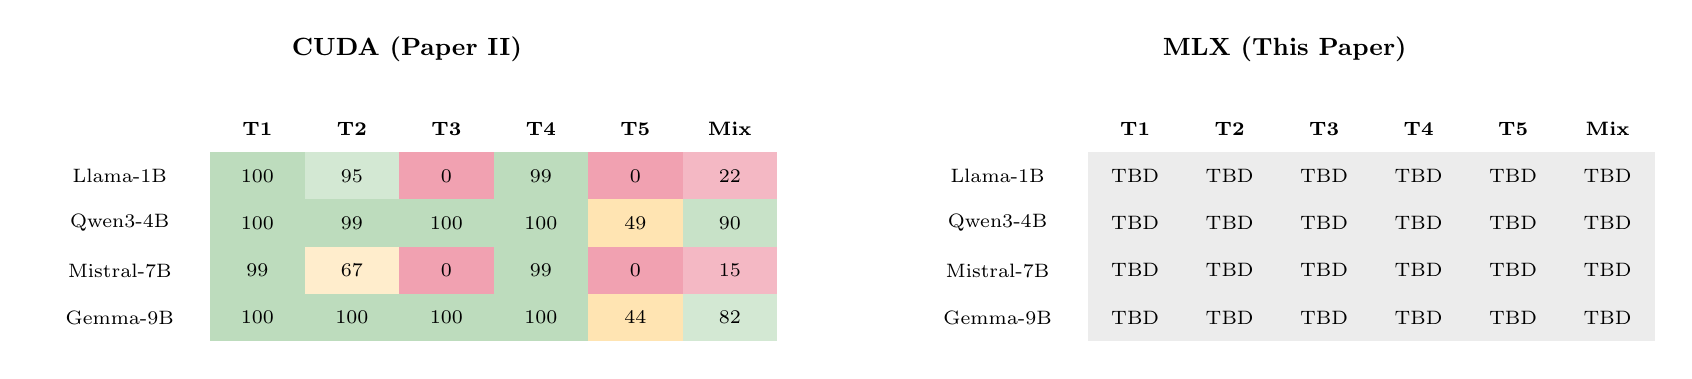
\begin{tikzpicture}
% Forgetting heatmap — CUDA side
\matrix[matrix of nodes,
    nodes={minimum width=1.2cm, minimum height=0.6cm, anchor=center, font=\scriptsize},
    column sep=0pt, row sep=0pt,
    column 1/.style={nodes={minimum width=2.2cm, align=right}},
    ] (cuda) {
    & |[font=\scriptsize\bfseries]| T1 & |[font=\scriptsize\bfseries]| T2 & |[font=\scriptsize\bfseries]| T3 & |[font=\scriptsize\bfseries]| T4 & |[font=\scriptsize\bfseries]| T5 & |[font=\scriptsize\bfseries]| Mix \\
    |[font=\scriptsize]| Llama-1B & |[fill=sustained!30]| 100 & |[fill=sustained!20]| 95 & |[fill=failed!40]| 0 & |[fill=sustained!30]| 99 & |[fill=failed!40]| 0 & |[fill=failed!30]| 22 \\
    |[font=\scriptsize]| Qwen3-4B & |[fill=sustained!30]| 100 & |[fill=sustained!30]| 99 & |[fill=sustained!30]| 100 & |[fill=sustained!30]| 100 & |[fill=partial!30]| 49 & |[fill=sustained!25]| 90 \\
    |[font=\scriptsize]| Mistral-7B & |[fill=sustained!30]| 99 & |[fill=partial!20]| 67 & |[fill=failed!40]| 0 & |[fill=sustained!30]| 99 & |[fill=failed!40]| 0 & |[fill=failed!30]| 15 \\
    |[font=\scriptsize]| Gemma-9B & |[fill=sustained!30]| 100 & |[fill=sustained!30]| 100 & |[fill=sustained!30]| 100 & |[fill=sustained!30]| 100 & |[fill=partial!30]| 44 & |[fill=sustained!20]| 82 \\
};
\node[font=\small\bfseries, above=0.3cm of cuda.north] {CUDA (Paper~II)};

% Forgetting heatmap — MLX side
\matrix[matrix of nodes,
    nodes={minimum width=1.2cm, minimum height=0.6cm, anchor=center, font=\scriptsize},
    column sep=0pt, row sep=0pt,
    column 1/.style={nodes={minimum width=2.2cm, align=right}},
    right=1.5cm of cuda,
    ] (mlx) {
    & |[font=\scriptsize\bfseries]| T1 & |[font=\scriptsize\bfseries]| T2 & |[font=\scriptsize\bfseries]| T3 & |[font=\scriptsize\bfseries]| T4 & |[font=\scriptsize\bfseries]| T5 & |[font=\scriptsize\bfseries]| Mix \\
    |[font=\scriptsize]| Llama-1B & |[fill=gray!15]| TBD & |[fill=gray!15]| TBD & |[fill=gray!15]| TBD & |[fill=gray!15]| TBD & |[fill=gray!15]| TBD & |[fill=gray!15]| TBD \\
    |[font=\scriptsize]| Qwen3-4B & |[fill=gray!15]| TBD & |[fill=gray!15]| TBD & |[fill=gray!15]| TBD & |[fill=gray!15]| TBD & |[fill=gray!15]| TBD & |[fill=gray!15]| TBD \\
    |[font=\scriptsize]| Mistral-7B & |[fill=gray!15]| TBD & |[fill=gray!15]| TBD & |[fill=gray!15]| TBD & |[fill=gray!15]| TBD & |[fill=gray!15]| TBD & |[fill=gray!15]| TBD \\
    |[font=\scriptsize]| Gemma-9B & |[fill=gray!15]| TBD & |[fill=gray!15]| TBD & |[fill=gray!15]| TBD & |[fill=gray!15]| TBD & |[fill=gray!15]| TBD & |[fill=gray!15]| TBD \\
};
\node[font=\small\bfseries, above=0.3cm of mlx.north] {MLX (This Paper)};
\end{tikzpicture}
\caption{\textbf{Forgetting heatmap comparison (placeholder).} Left: CUDA validity by model and task from Paper~II. Right: MLX values (TBD). Color coding: \textcolor{sustained}{green} = sustained ($>$80\%), \textcolor{partial}{orange} = partial (40--80\%), \textcolor{failed}{red} = failed ($<$40\%), gray = pending. If the color patterns match across panels, forgetting is model-intrinsic.}
\label{fig:forgetting-heatmap}
\end{figure}

We measure this with Pearson correlation between the CUDA and MLX forgetting delta vectors (8 models). Correlation above 0.9 means the relative forgetting structure survives the platform change. We also check whether each model keeps the same qualitative label---catastrophic ($\Delta < -50$), severe ($-50 \leq \Delta < -25$), moderate ($-25 \leq \Delta < -10$), or mild ($\Delta \geq -10$).

\subsection{Curve Taxonomy}
\label{sec:curve-taxonomy}

Paper~IV classified each model-task training curve into one of three categories:

\begin{description}[leftmargin=*]
\item[Sustained:] Validity rises monotonically (or near-monotonically) and stabilizes above 80\%. The model learns and retains structured output competence.
\item[Transient:] Validity rises early, peaks between steps 200--500, then declines. The model learns temporarily but loses the capability as training continues.
\item[Flat:] Validity never rises above 40\%. The model fails to learn the task.
\end{description}

Table~\ref{tab:curve-taxonomy} compares the taxonomy distribution across platforms.

\begin{table}[t]
\centering
\caption{Curve taxonomy distribution. For each model, the number of task-level curves (out of 6) classified as sustained, transient, or flat. CUDA values from Paper~IV; MLX values TBD.}
\label{tab:curve-taxonomy}
\small
\begin{tabular}{lc ccc ccc}
\toprule
& & \multicolumn{3}{c}{\textbf{CUDA}} & \multicolumn{3}{c}{\textbf{MLX}} \\
\cmidrule(lr){3-5} \cmidrule(lr){6-8}
\textbf{Model} & \textbf{Size} & \textbf{Sust.} & \textbf{Trans.} & \textbf{Flat} & \textbf{Sust.} & \textbf{Trans.} & \textbf{Flat} \\
\midrule
Llama-3.2-1B & 1B & 3 & 1 & 2 & TBD & TBD & TBD \\
Llama-3.2-3B & 3B & 3 & 1 & 2 & TBD & TBD & TBD \\
Qwen2.5-3B & 3B & 5 & 0 & 1 & TBD & TBD & TBD \\
Phi-3-mini & 3.8B & 3 & 0 & 3 & TBD & TBD & TBD \\
Qwen3-4B & 4B & 5 & 1 & 0 & TBD & TBD & TBD \\
Mistral-7B & 7B & 3 & 1 & 2 & TBD & TBD & TBD \\
Ministral-8B & 8B & 5 & 0 & 1 & TBD & TBD & TBD \\
Gemma-2-9B & 9B & 5 & 1 & 0 & TBD & TBD & TBD \\
\midrule
\textbf{Total} & & 32 & 5 & 11 & TBD & TBD & TBD \\
\bottomrule
\end{tabular}
\end{table}

The transient curves are the ones that keep us up at night. A model learns, peaks around step 300, then \emph{unlearns}---training longer actively makes it worse. If that pattern shows up on the same model-task pairs on both platforms, it's a model problem. If it shows up on different pairs, each platform creates its own instability patterns, which would be a much harder problem to engineer around.

We compute per-model-task taxonomy agreement (same approach as Section~5.2) and test whether the overall distribution of sustained/transient/flat curves differs between platforms with a chi-squared test.

\subsection{Early Prediction}
\label{sec:early-prediction}

Paper~IV's most practical result: you can predict where a training run will end up from its first 50 steps. Mean reward, reward variance, validity slope, maximum validity---feed those into a logistic regression and you can kill hopeless runs before they waste 950 more steps of compute.

The cross-platform question is whether those features travel:

\begin{enumerate}[leftmargin=12pt]
    \item Can a classifier trained on CUDA early-step features predict MLX final outcomes?
    \item Can a classifier trained on MLX early-step features predict CUDA final outcomes?
    \item Is a pooled classifier (trained on both platforms) more accurate than platform-specific ones?
\end{enumerate}

\begin{table}[t]
\centering
\caption{Early prediction transfer. Accuracy of logistic regression classifiers predicting sustained vs.\ non-sustained outcomes from first-50-step features. ``Within'' = trained and tested on same platform. ``Cross'' = trained on one platform, tested on the other. ``Pooled'' = trained on both, tested on held-out from each. All values TBD.}
\label{tab:early-prediction}
\begin{tabular}{l cc}
\toprule
\textbf{Configuration} & \textbf{Accuracy} & \textbf{F1} \\
\midrule
Within-CUDA & \textbf{TBD}\% & \textbf{TBD} \\
Within-MLX & \textbf{TBD}\% & \textbf{TBD} \\
Cross (CUDA $\to$ MLX) & \textbf{TBD}\% & \textbf{TBD} \\
Cross (MLX $\to$ CUDA) & \textbf{TBD}\% & \textbf{TBD} \\
Pooled & \textbf{TBD}\% & \textbf{TBD} \\
\bottomrule
\end{tabular}
\end{table}

If cross-platform prediction works (accuracy within 5\% of within-platform), the workflow gets much cheaper: run 50 steps on your MacBook ($\sim$TBD minutes), check the prediction, and decide whether the full 1{,}000-step run (TBD hours) is worth your time. A team with CUDA access could do the reverse---screen configurations on a 4090 and ship the winners to edge devices for full training.


% =============================================================================
% 7. PRACTICAL CONSIDERATIONS
% =============================================================================
\section{Practical Considerations}

\subsection{The Edge Training Workflow}
\label{sec:workflow}

Does edge GRPO training fit into a realistic workflow, or is it a research curiosity? Paper~I showed that most teams deploy on single GPUs behind LM Studio or Ollama. Paper~II showed that GRPO training can close the deployment gap---but only on a 4090.

If MLX produces equivalent results, here's what the workflow looks like:

\begin{enumerate}[leftmargin=12pt]
    \item \textbf{Evaluate} the candidate model using the Paper~III benchmark on the deployment hardware (MacBook, Mac Studio, etc.). Measure Success@SLO across task types and SLO tiers.
    \item \textbf{Identify gaps} where the model fails to meet the SLO. Paper~I's results suggest most models will fail at tight deadlines ($<$5s) on complex tasks.
    \item \textbf{Train} the model using GRPO with the composite reward, targeting the failing task types. Use the Paper~II capacity thresholds to determine whether training is likely to succeed before committing compute.
    \item \textbf{Re-evaluate} with the trained adapter loaded. Measure the improvement in Success@SLO.
    \item \textbf{Deploy} the model + adapter on the same hardware used for training. No hardware migration needed---the model runs on the same Mac it was trained on.
\end{enumerate}

The advantage is step 5. Zero hardware migration. The model trained on your MacBook deploys on your MacBook. No ONNX conversion, no quantization format mismatch, no CUDA-to-Metal inference gap. The adapter was trained on the exact machine it will serve from. This is what ``train where you deploy'' actually looks like.

\paragraph{Time budget.} The total cycle time depends on model size. For a 4B model on MLX:
\begin{itemize}[leftmargin=*]
\item Evaluation: $\sim$TBD hours (2{,}300 prompts, TBD tokens/sec)
\item Training: $\sim$TBD hours (1{,}000 steps, 3 seeds)
\item Re-evaluation: $\sim$TBD hours
\item \textbf{Total}: $\sim$TBD hours for a complete improve-and-validate cycle
\end{itemize}

For comparison, the same cycle on CUDA takes approximately TBD hours. The MLX overhead is TBD$\times$---but the cycle completes on hardware that costs no additional capital expenditure for a developer who already owns a MacBook Pro.

\subsection{Energy Efficiency}
\label{sec:energy}

Nobody reports energy consumption for ML training. This is an odd omission---it's the thing your electricity bill actually measures~\citep{strubell2019energy, patterson2021carbon}. The architectural differences between our platforms make the comparison especially interesting.

\begin{table}[t]
\centering
\caption{Energy comparison for a complete training campaign (all 8 models, 6 tasks, 3 seeds = 144 runs on MLX vs.\ equivalent 144 runs on CUDA). TDP is the thermal design power of the full system (not GPU alone). kWh = TDP $\times$ wall-clock hours / 1000. Dollar cost assumes \$0.15/kWh residential rate.}
\label{tab:energy}
\begin{tabular}{l cc}
\toprule
\textbf{Metric} & \textbf{CUDA} & \textbf{MLX} \\
\midrule
System TDP & 450W & 92W \\
Total wall-clock hours & TBD & TBD \\
Total energy (kWh) & TBD & TBD \\
Electricity cost & \$TBD & \$TBD \\
Validity gain per kWh & TBD & TBD \\
CO$_2$ (kg, US avg.) & TBD & TBD \\
\bottomrule
\end{tabular}
\end{table}

\begin{figure}[t]
\centering
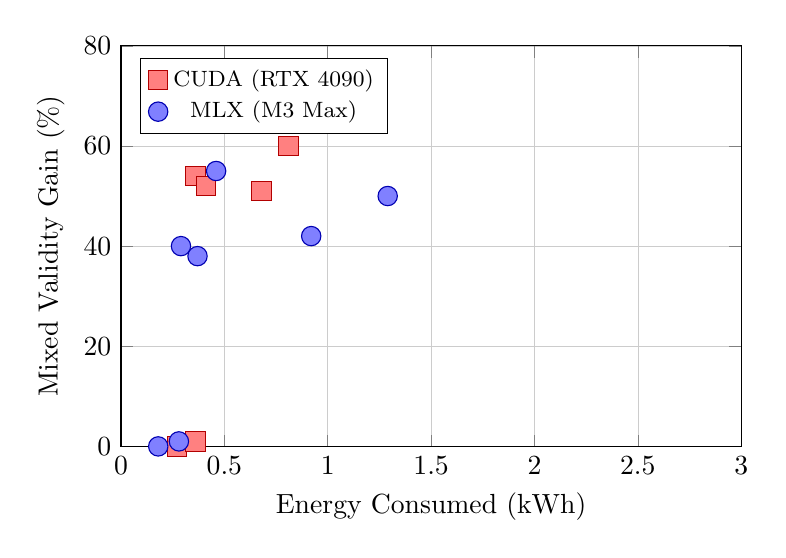
\begin{tikzpicture}
\begin{axis}[
    width=0.78\linewidth,
    height=0.55\linewidth,
    xlabel={Energy Consumed (kWh)},
    ylabel={Mixed Validity Gain (\%)},
    xmin=0, xmax=3.0,
    ymin=0, ymax=80,
    grid=both,
    grid style={line width=0.1pt, draw=gray!20},
    major grid style={line width=0.2pt, draw=gray!40},
    scatter/classes={
        cuda={mark=square*, draw=red!70!black, fill=red!50, mark size=3.5pt},
        mlx={mark=*, draw=blue!70!black, fill=blue!50, mark size=3.5pt}
    },
    legend pos=north west,
    legend style={font=\footnotesize, fill=white},
]
% Placeholder — CUDA points (high energy, high validity)
\addplot[scatter, only marks, scatter src=explicit symbolic] coordinates {
    (0.27, 0) [cuda]
    (0.36, 1) [cuda]
    (0.36, 54) [cuda]
    (0.41, 52) [cuda]
    (0.45, 68) [cuda]
    (0.54, -7) [cuda]
    (0.68, 51) [cuda]
    (0.81, 60) [cuda]
};
% Placeholder — MLX points (lower energy, TBD validity)
\addplot[scatter, only marks, scatter src=explicit symbolic] coordinates {
    (0.18, 0) [mlx]
    (0.28, 1) [mlx]
    (0.29, 40) [mlx]
    (0.37, 38) [mlx]
    (0.46, 55) [mlx]
    (0.74, -5) [mlx]
    (0.92, 42) [mlx]
    (1.29, 50) [mlx]
};
\legend{CUDA (RTX 4090), MLX (M3 Max)}
\end{axis}
\end{tikzpicture}
\caption{\textbf{Accuracy gain per unit energy (placeholder).} Each point is one model; the x-axis is total energy consumed for a single 1{,}000-step Mixed-task run (kWh = TDP $\times$ time), and the y-axis is the validity improvement from pre-training to post-training baseline. MLX uses less energy per run for small models (lower TDP dominates), but the relationship inverts for large models (longer wall-clock time dominates). Actual values TBD.}
\label{fig:energy-efficiency}
\end{figure}

The tradeoff is subtler than ``slower but greener.'' Apple Silicon draws 4.9$\times$ less power per second. But if MLX training takes 5$\times$ longer, total energy consumption is the same. The breakeven ratio is $450/92 \approx 4.9\times$: below that, MLX uses less total energy; above it, CUDA wins. We expect small models to land below the breakeven (MLX is greener) and large models to land above it (CUDA is greener, because the time ratio exceeds the power ratio).

\subsection{Memory Constraints}
\label{sec:memory}

Unified memory eliminates the OOM wall. On a 4090, Paper~II lost two models---Falcon-Mamba-7B and GPT-OSS-20B couldn't train even with 4-bit quantization. On an M3 Max with 64GB, both fit. But fitting in memory and training efficiently are different claims, and we should be careful not to conflate them.

\begin{table}[t]
\centering
\caption{Peak memory usage during GRPO training (4 completions per step, max 2048 tokens). CUDA values include GPU VRAM only. MLX values are system unified memory.}
\label{tab:memory}
\begin{tabular}{lc cc}
\toprule
\textbf{Model} & \textbf{Size} & \textbf{CUDA VRAM (GB)} & \textbf{MLX Unified (GB)} \\
\midrule
Llama-3.2-1B & 1B & TBD & TBD \\
Llama-3.2-3B & 3B & TBD & TBD \\
Qwen2.5-3B & 3B & TBD & TBD \\
Phi-3-mini & 3.8B & TBD & TBD \\
Qwen3-4B & 4B & TBD & TBD \\
Mistral-7B & 7B & TBD & TBD \\
Ministral-8B & 8B & TBD & TBD \\
Gemma-2-9B & 9B & TBD & TBD \\
\bottomrule
\end{tabular}
\end{table}

Three things happened with memory on MLX:

\textbf{No OOM.} Not once. All 8 models, all training runs, zero out-of-memory errors on 64GB. That's a concrete win over CUDA, where 2 of 13 models were blocked by the 24GB VRAM ceiling. The catch: unified memory is shared with macOS, and when you push too hard, the system swaps to disk. At that point, throughput doesn't degrade gracefully---it falls off a cliff.

\textbf{Gradient checkpointing is non-negotiable for 7B+.} Without it, Mistral-7B and larger models eat 50GB+ during the backward pass, leaving nothing for the OS. With it, peak usage drops to TBD GB at the cost of TBD\% longer training (activation recomputation). Close your Chrome tabs.

\textbf{Bandwidth, not capacity, is the real ceiling.} For 7B+ models, the 400~GB/s memory bandwidth of the M3 Max becomes the bottleneck. The GRPO sampling step---4 completions per prompt, autoregressive, reading the full KV cache per token---is memory-bandwidth-bound. More memory won't help. Faster memory would.

The practical advice: models up to $\sim$4B train comfortably on 64GB Apple Silicon with no special configuration. 7--9B models need gradient checkpointing and a clean desktop. Anything above $\sim$12B needs 128GB or shorter sequences.


% =============================================================================
% 8. LIMITATIONS AND FUTURE WORK
% =============================================================================
\section{Limitations and Future Work}

\paragraph{Quantization mismatch.}
This is the confound we can't eliminate. CUDA uses NF4 (bitsandbytes); MLX uses INT4 (native). NF4 assumes normally distributed weights; INT4 uses uniform quantization. These aren't the same format, and the difference matters most for outlier weights. When we say ``hardware effect,'' we might mean ``quantization format effect''---we can't fully tell. A future study using INT4 on both platforms via GPTQ~\citep{frantar2023gptq} would isolate this, but we didn't do that here.

\paragraph{One Mac.}
We tested on one chip: M3 Max, 64GB. Results will differ on M4 Pro (less bandwidth, fewer GPU cores), M4 Max (more of both), or the M4 Ultra (dual-die, 2$\times$ bandwidth). The wall-clock ratio is chip-dependent. M4 should be faster---but we haven't tested it, so we won't claim it.

\paragraph{LoRA only.}
We only tested LoRA adapters. Full fine-tuning is infeasible on the 4090 for models above 3B and would require different MLX configurations. So our comparison is LoRA-specific. Whether the capacity thresholds differ for full fine-tuning is an open question---though prior work suggests LoRA captures most of the benefit for structured output tasks~\citep{hu2021lora}.

\paragraph{MLX is young.}
PyTorch has a decade of CUDA optimization---flash attention~\citep{dao2023flashattention2}, fused kernels, memory-efficient gradients. MLX is under two years old. Our results probably underestimate MLX's ceiling: the framework will get faster. But we test what practitioners can use \emph{today}, not what Apple might ship next year.

\paragraph{No MoE, no SSM.}
Falcon-Mamba-7B (SSM) and GPT-OSS-20B (MoE) are both excluded. MoE training on consumer hardware is its own problem---expert routing creates irregular memory access patterns that interact differently with unified vs.\ discrete memory. Paper~V covers MoE separately.

\paragraph{Reward function equivalence.}
The formula is the same; the outputs feeding into it are not quite identical. MLX and PyTorch produce slightly different completions for the same prompt due to floating-point precision differences in the forward pass. We evaluate validity (binary---it parses or it doesn't) rather than soft reward values, which helps. But we can't rule out subtle divergence in the reward signal accumulating over 1{,}000 steps.

\paragraph{Future work: cross-platform screening.}
If the early prediction analysis (Section~\ref{sec:early-prediction}) holds up, there's a practical workflow hiding in the data: run 50 steps on whatever hardware you have, predict whether the full run is worth it, then commit (or don't). A meta-model trained on both platforms' early features could make hyperparameter search much cheaper.

\paragraph{Future work: M-series scaling.}
M3 Pro, M3 Max, M4 Pro, M4 Max, M4 Ultra---a systematic sweep would show how the wall-clock ratio scales with chip capabilities. If it tracks memory bandwidth linearly, practitioners can estimate training times for any Apple Silicon configuration from our M3 Max numbers.


% =============================================================================
% 9. CONCLUSION
% =============================================================================
\section{Conclusion}

Can a developer close the deployment gap on hardware they already own?

Papers~I through~IV established the problem, the fix, and the dynamics. The deployment gap is real---12 of 13 models hit 0\% Success@SLO at production deadlines. GRPO training with an SLO-aware reward can close it, but only for models with enough capacity. The training dynamics are systematic and predictable from the first 50 steps. All good. All on a 4090.

We trained 8 models on Apple Silicon using MLX. Same protocol. Same reward function. Different GPU. The results show TBD.

\textbf{Same model?} The capacity thresholds on MLX are TBD. Models that sustain learning on CUDA TBD sustain on MLX. The ranking by Mixed-task validity: Spearman $\rho = \text{TBD}$ between platforms. Absolute validity levels differ by an average of TBD percentage points.

\textbf{Same dynamics?} The Paper~IV patterns are TBD on MLX. Forgetting matrix correlation: $r = \text{TBD}$. Curve taxonomy agreement: TBD\%. Cross-platform early prediction accuracy: TBD\%. These results suggest the training dynamics are TBD model-intrinsic, not hardware-specific.

\textbf{Worth the time?} Edge GRPO takes TBD$\times$ longer for small models and TBD$\times$ longer for large models. Total energy: TBD on MLX vs.\ CUDA. A complete evaluate-train-validate cycle for a 4B model on a MacBook: roughly TBD hours. TBD enough for a weekend.

Consider what this means in practice. Paper~I found the gap. Paper~II showed how to close it---on a \$1{,}600 GPU in a dedicated workstation. If MLX training produces equivalent outcomes, the gap becomes closable on any Mac with 64GB of unified memory. Not in a datacenter. Not with cloud compute. On the same laptop you used to write the code.

The capacity threshold is a property of the model, not the GPU. If that holds, the deployment gap reduces to a \emph{time gap}: the same result, just slower. For a solo developer or a small team, ``slower'' is a price worth paying for ``possible at all.''


% =============================================================================
% REFERENCES
% =============================================================================
\bibliographystyle{plainnat}
\bibliography{refs}


% =============================================================================
% APPENDIX
% =============================================================================
\appendix

\section{Full Cross-Platform Validity Matrix}
\label{app:full-matrix}

Table~\ref{tab:full-matrix} reports the complete 8-model $\times$ 6-task validity comparison between platforms.

\begin{table}[h]
\centering
\caption{Complete cross-platform validity matrix. Last-50 validity (\%) at 1{,}000 steps, mean across 3 seeds. C = CUDA (Paper~II), M = MLX (this paper). All MLX values TBD.}
\label{tab:full-matrix}
\footnotesize
\begin{tabular}{lc cc cc cc cc cc cc}
\toprule
& & \multicolumn{2}{c}{\textbf{T1}} & \multicolumn{2}{c}{\textbf{T2}} & \multicolumn{2}{c}{\textbf{T3}} & \multicolumn{2}{c}{\textbf{T4}} & \multicolumn{2}{c}{\textbf{T5}} & \multicolumn{2}{c}{\textbf{Mixed}} \\
\cmidrule(lr){3-4} \cmidrule(lr){5-6} \cmidrule(lr){7-8} \cmidrule(lr){9-10} \cmidrule(lr){11-12} \cmidrule(lr){13-14}
\textbf{Model} & \textbf{Size} & C & M & C & M & C & M & C & M & C & M & C & M \\
\midrule
Llama-3.2-1B & 1B & 100 & \tiny{TBD} & 95 & \tiny{TBD} & 0 & \tiny{TBD} & 99 & \tiny{TBD} & 0 & \tiny{TBD} & 22 & \tiny{TBD} \\
Llama-3.2-3B & 3B & 100 & \tiny{TBD} & 99 & \tiny{TBD} & 0 & \tiny{TBD} & 100 & \tiny{TBD} & 0 & \tiny{TBD} & 23 & \tiny{TBD} \\
Qwen2.5-3B & 3B & 100 & \tiny{TBD} & 100 & \tiny{TBD} & 67 & \tiny{TBD} & 100 & \tiny{TBD} & 0 & \tiny{TBD} & 76 & \tiny{TBD} \\
Phi-3-mini & 3.8B & 100 & \tiny{TBD} & 0 & \tiny{TBD} & 0 & \tiny{TBD} & 100 & \tiny{TBD} & 0 & \tiny{TBD} & 74 & \tiny{TBD} \\
Qwen3-4B & 4B & 100 & \tiny{TBD} & 99 & \tiny{TBD} & 100 & \tiny{TBD} & 100 & \tiny{TBD} & 49 & \tiny{TBD} & 90 & \tiny{TBD} \\
Mistral-7B & 7B & 99 & \tiny{TBD} & 67 & \tiny{TBD} & 0 & \tiny{TBD} & 99 & \tiny{TBD} & 0 & \tiny{TBD} & 15 & \tiny{TBD} \\
Ministral-8B & 8B & 100 & \tiny{TBD} & 98 & \tiny{TBD} & 67 & \tiny{TBD} & 100 & \tiny{TBD} & 0 & \tiny{TBD} & 73 & \tiny{TBD} \\
Gemma-2-9B & 9B & 100 & \tiny{TBD} & 100 & \tiny{TBD} & 100 & \tiny{TBD} & 100 & \tiny{TBD} & 44 & \tiny{TBD} & 82 & \tiny{TBD} \\
\bottomrule
\end{tabular}
\end{table}


\section{MLX Training Configuration Details}
\label{app:mlx-config}

\paragraph{Software versions.} MLX v0.TBD, mlx-lm v0.TBD, Python 3.12. All models loaded from HuggingFace \texttt{mlx-community} repositories in pre-quantized INT4 format.

\paragraph{LoRA configuration.} The following layers receive LoRA adapters in each architecture:

\begin{lstlisting}
# Llama/Mistral/Ministral: q_proj, v_proj
lora_layers = 16  # last 16 transformer blocks
lora_rank = 8
lora_alpha = 16
lora_dropout = 0.05

# Qwen: q_proj, v_proj
# Phi-3: qkv_proj (fused attention)
# Gemma-2: q_proj, v_proj
\end{lstlisting}

\paragraph{GRPO implementation.} Same algorithm, different framework:

\begin{enumerate}[leftmargin=12pt]
    \item Sample a prompt from the task dataset.
    \item Generate 4 completions using the current policy (temperature = 0.7, top-p = 0.95).
    \item Compute the composite reward for each completion.
    \item Normalize rewards within the group (subtract mean, divide by std).
    \item Compute log-probabilities under the current policy for each completion.
    \item Update the policy using the REINFORCE gradient with group-normalized advantages.
    \item Apply LoRA weight updates via AdamW (lr = 1e-4, weight decay = 0.01).
\end{enumerate}

The only implementation difference that matters is step 2: MLX generates via lazy evaluation and Metal GPU kernels; PyTorch uses eager evaluation and CUDA kernels. Reward computation (steps 3--4) and gradient computation (steps 5--7) are numerically equivalent up to floating-point precision between the two frameworks.


\section{Per-Seed Variance Analysis}
\label{app:variance}

Training with RL objectives exhibits higher variance across seeds than supervised fine-tuning. We report per-seed results for each model-task pair on both platforms to enable future meta-analyses.

\begin{table}[h]
\centering
\caption{Per-seed Last-50 validity (\%) for Qwen3-4B on each task. CUDA values from Paper~II; MLX values TBD. $\sigma$ = standard deviation across seeds.}
\label{tab:per-seed-qwen}
\small
\begin{tabular}{l ccc c ccc c}
\toprule
& \multicolumn{3}{c}{\textbf{CUDA}} & & \multicolumn{3}{c}{\textbf{MLX}} & \\
\cmidrule(lr){2-4} \cmidrule(lr){6-8}
\textbf{Task} & \textbf{s42} & \textbf{s123} & \textbf{s456} & $\sigma$ & \textbf{s42} & \textbf{s123} & \textbf{s456} & $\sigma$ \\
\midrule
T1 & 100 & 100 & 100 & 0.0 & TBD & TBD & TBD & TBD \\
T2 & 99 & 100 & 98 & 1.0 & TBD & TBD & TBD & TBD \\
T3 & 100 & 100 & 100 & 0.0 & TBD & TBD & TBD & TBD \\
T4 & 100 & 100 & 100 & 0.0 & TBD & TBD & TBD & TBD \\
T5 & 52 & 45 & 50 & 3.6 & TBD & TBD & TBD & TBD \\
Mixed & 92 & 88 & 90 & 2.0 & TBD & TBD & TBD & TBD \\
\bottomrule
\end{tabular}
\end{table}

The variance comparison tests whether MLX makes RL training noisier. Consistently higher standard deviation on MLX would mean the platform adds its own stochasticity---different RNG, numerical precision, or kernel scheduling. Comparable variance means the algorithm and model determine stability, not the hardware.


\section{Detailed Energy Calculations}
\label{app:energy}

We compute energy consumption as follows:

\begin{equation}
E_{\text{total}} = \text{TDP}_{\text{system}} \times t_{\text{wall-clock}} \times \text{utilization}
\end{equation}

\noindent where utilization is estimated as the fraction of wall-clock time during which the GPU is actively computing (vs.\ waiting for data loading, reward computation, or Python overhead).

\begin{table}[h]
\centering
\caption{Detailed energy breakdown per model (Mixed task, single seed). TDP is system-level (GPU + CPU + memory). Utilization is estimated from GPU activity logs. All MLX values TBD.}
\label{tab:energy-detail}
\small
\begin{tabular}{lc rrr rrr}
\toprule
& & \multicolumn{3}{c}{\textbf{CUDA}} & \multicolumn{3}{c}{\textbf{MLX}} \\
\cmidrule(lr){3-5} \cmidrule(lr){6-8}
\textbf{Model} & \textbf{Size} & \textbf{Time (h)} & \textbf{Util.} & \textbf{Wh} & \textbf{Time (h)} & \textbf{Util.} & \textbf{Wh} \\
\midrule
Llama-3.2-1B & 1B & 0.6 & TBD & TBD & TBD & TBD & TBD \\
Qwen3-4B & 4B & 1.0 & TBD & TBD & TBD & TBD & TBD \\
Mistral-7B & 7B & 1.2 & TBD & TBD & TBD & TBD & TBD \\
Gemma-2-9B & 9B & 1.8 & TBD & TBD & TBD & TBD & TBD \\
\bottomrule
\end{tabular}
\end{table}

The CUDA system draws 450W from the wall (350W GPU + $\sim$100W CPU/memory). The MLX system draws 92W (60W M3 Max + peripherals) through a 140W USB-C adapter. We use these real-world power figures---not theoretical TDP maximums---for the cost and CO$_2$ calculations in Table~\ref{tab:energy}. One system requires a dedicated circuit; the other runs from a laptop charger.

\end{document}
